\documentclass{article}
    % General document formatting
    \usepackage[margin=0.7in]{geometry}
    \usepackage[parfill]{parskip}
    \usepackage[utf8]{inputenc}
    
    % Related to math
    \usepackage{amsmath,amssymb,amsfonts,amsthm}
\usepackage{graphicx}
%\usepackage{subfig}
%\usepackage{subfigure}
\usepackage{caption}
\usepackage{subcaption}
\usepackage{listings}
\usepackage{braket}
\usepackage{gensymb}
\usepackage[percent]{overpic}
\usepackage{xcolor,varwidth}

\usepackage{titling}
%\usepackage{lipsum}

\usepackage{titlesec}

\titleformat*{\section}{\Large\bfseries}
\titleformat*{\subsection}{\large\bfseries}
%\titleformat*{\subsubsection}{\large\bfseries}
%\titleformat*{\paragraph}{\large\bfseries}
%\titleformat*{\subparagraph}{\large\bfseries}
\titlespacing\section{0pt}{12pt plus 4pt minus 2pt}{0pt plus 2pt minus 2pt}
\titlespacing\subsection{0pt}{12pt plus 4pt minus 2pt}{0pt plus 2pt minus 2pt}
\titlespacing\subsubsection{0pt}{12pt plus 4pt minus 2pt}{0pt plus 2pt minus 2pt}

\pretitle{\begin{center}\large\bfseries}
\posttitle{\par\end{center}\vskip 0.01em}
\preauthor{\begin{center}\Large\ttfamily}
\postauthor{\end{center}}
\predate{\par\normalsize\centering}
\postdate{\par}

\title{Population Genetic Analyses of Genomic Data 1}
%\date{\today}


\begin{document}

%\maketitle

\begin{center}
\textbf{\LARGE{\centering{Cancer Evolution 2}}}\\

\textit{USN: 303039534}\\
\end{center}

\section*{A}

\subsection*{1}

We label the aquired mutations and clones as illustrated in figure \ref{fig:tree2}. We then note from figure \ref{fig:tree1} that the healthy cell population represents $\pi_0 = 2/12$ of the total cell population. The cancer cell fraction for a given set of mutations $i$ emerging in clone $k$ is thus given by 
\begin{equation}
\tau_i = \dfrac{N_i}{N_{cancer}} = \dfrac{12}{10} \tau_i^{cell}   = \dfrac{12}{10} \sum_{I \in \text{de}(k)}{\pi_I}
\end{equation}
Where $\tau_i^{cell}$ is the cell fraction of mutation $i$ and $\pi_I$ is the clonal frequency of clone $I$ with all clonal frequencies given in figure \ref{fig:tree1}.

\begin{figure}[h]
	\centering
	\begin{subfigure}[t]{0.18\linewidth}
		\centering
		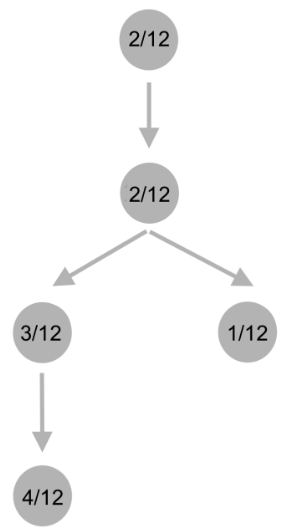
\includegraphics[width = 1.0\linewidth, trim={0 0 0 0}, clip=true]{tree1.png}
		\subcaption{Phylogenetic tree and clonal frequencies of the tumor given in the assignment.}
		\label{fig:tree1}	
	\end{subfigure}%
	\hspace{0.15 \linewidth}
	\begin{subfigure}[t]{0.29\linewidth}
		\centering
		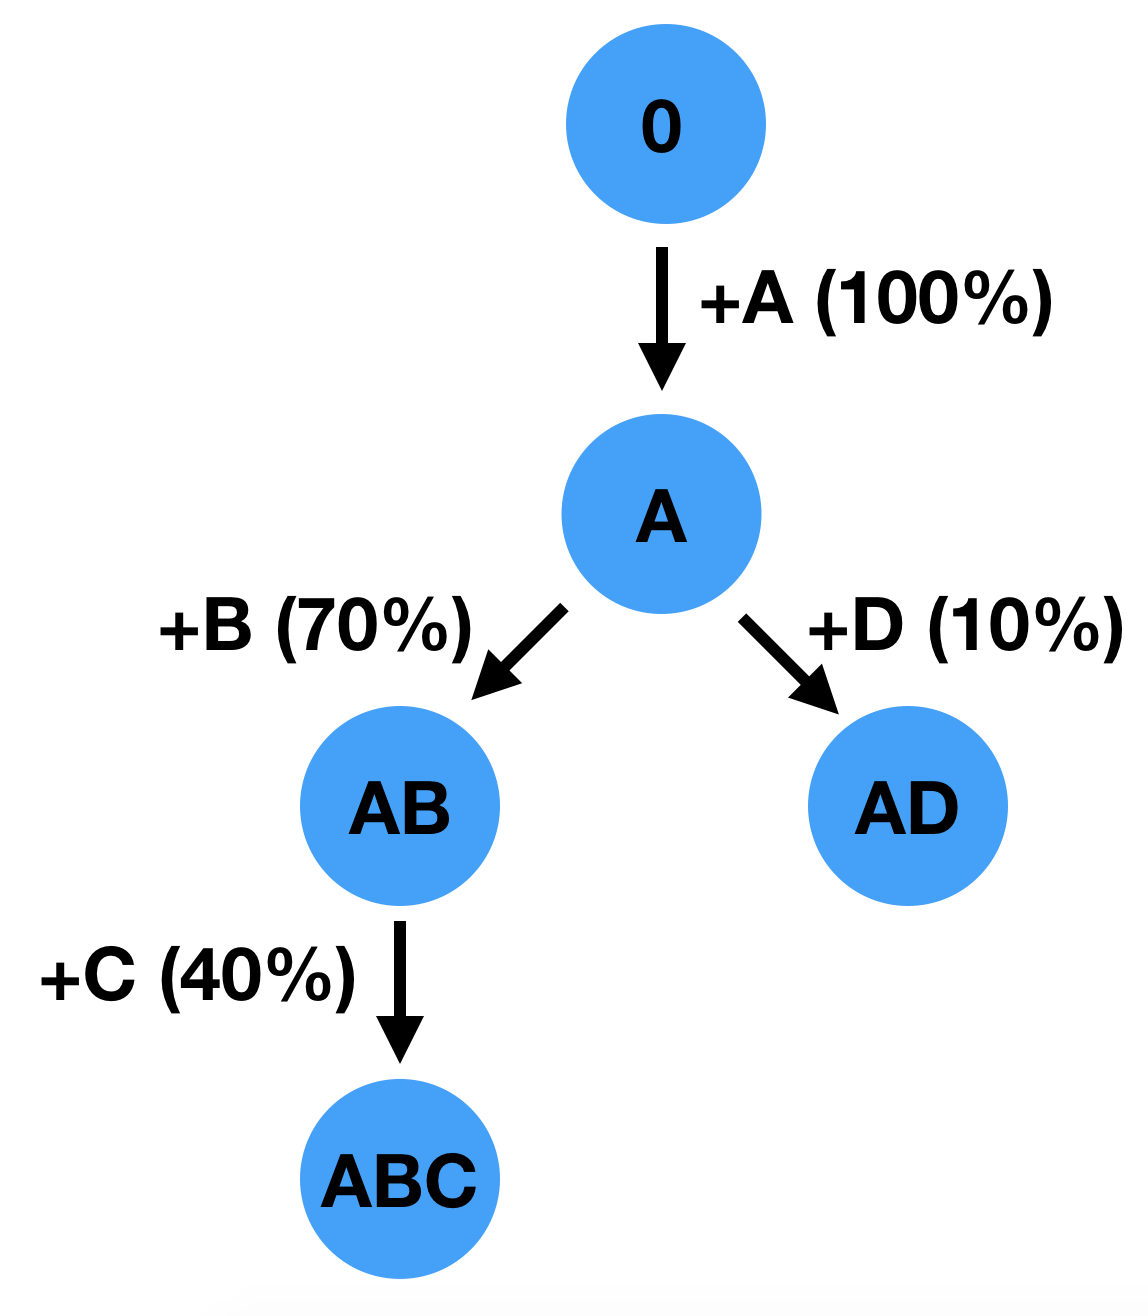
\includegraphics[width = 1.0\linewidth, trim={0 0 0 0}, clip=true]{tree2.png}
		\subcaption{Phylogenetic tree with mutations and clones labelled. Cancer cell fractions are given in brackets next to the edge at which a given set of mutations is acquired.}
		\label{fig:tree2}	
	\end{subfigure}%
\caption{Tumor phylogenetic trees illustrating clonal frequencies (left) and cancer cell fractions (right).}
\label{fig:tree}
\end{figure}

The cancer cell fractions are thus given by [100\%, 70\%, 40\%, 10\%] corresponding to cellular frequencies of [83.3\%, 58.3\%, 33.3\%, 8.3\%].

\subsection*{2}

PyClone and Ccube were installed as specfied in their documentation and run with default parameters unless otherwise stated. All calculations were run on subliminal to make runtimes comparable.

In table \ref{tab:perf} we report both the runtimes and inferred number of clusters of CCFs for both methods.
We note that the runtime for Ccube depends on the maximum number of clusters considered (\textit{numOfClusterPool}) and is super-linear in this parameter. We therefore report runtimes considering both numOfClusterPool=1:6 as in the vignette and numOfClusterPool=1:11 since the maximum number of possible clusters is 11 (see section 5).
 

\begin{table}[h]
\centering
\begin{tabular}{ |c|c|c|c|c|c|c|}
\hline
 & PyClone 0\% & PyClone 70\% & Ccube 0\% (6) & Ccube 70\% (6)& Ccube 0\% (11) & Ccube 70\% (11) \\
\hline
runtime (s) &  1071.04  & 1886.60 & 4.32 & 10.49 & 15.58 &  23.69\\
clusters & 20 & 67 & 4 & 4 & 4 & 5\\
clusters ($>1$) & 4 & 6 & 4 & 4 & 4 & 5\\
\hline
\end{tabular}
\caption{Runtime and inferred cluster counts for PyClone and Ccube. "0\%" indicates data with no copy number changes and "70\%" indicates data with copy number changes at 70\% of loci. The number in brackets for the Ccube calculations specifies the maximum number of clusters considered in the algorithm. The third line indicates the number of clusters assigned more than one mutation.}
\label{tab:perf}
\end{table}

We see that the runtime for PyClone is generally much higher than that for Ccube, even when allowing for up to 11 clusters in Ccube. This will be discussed further below. We also note that the runtime for PyClone increases by 76\% when including copy number variation whereas it only increases by 50\% when considering up to 11 clusters in Ccube. When only considering up to 6 mutations in Ccube, the runtime increases by 150\% when including copy number variation, but the runtime is more than two orders of magnitude faster than PyClone in this case.

\subsection*{3}

The number of inferred mutations for each calculation is also given in table \ref{tab:perf}. PyClone often found clusters of singletons which may arise primarily due to noise, and we therefore also report in the third row of the table the number of CCF clusters found for which the mutation count is greater than 1.

We see that when considering only these non-singleton clusters, both PyClone and Ccube correctly infer 4 CCF clusters. However, Ccube does so much more quickly and without the additional singleton clusters from PyClone. In addition, Ccube correctly identifies 4 clusters even in the presence of 70\% copy number variation when allowing up to 6 clusters, although it identifies 5 clusters when allowing up to 11 clusters. In this case, PyClone incorrectly infers 6 clusters.

To further compare the inferred CCF clusters with the real CCF clusters, we plot in figure \ref{fig:pyclone} the real and inferred cancer cell fractions in a format similar to the 'column summary' from assignment 1. Note that the bar heights are arbitrary for the reference data as we are not given information on how many mutations were simulated for each clone.

\begin{figure}[h]
	\centering
	\begin{subfigure}[t]{0.32\linewidth}
		\centering
		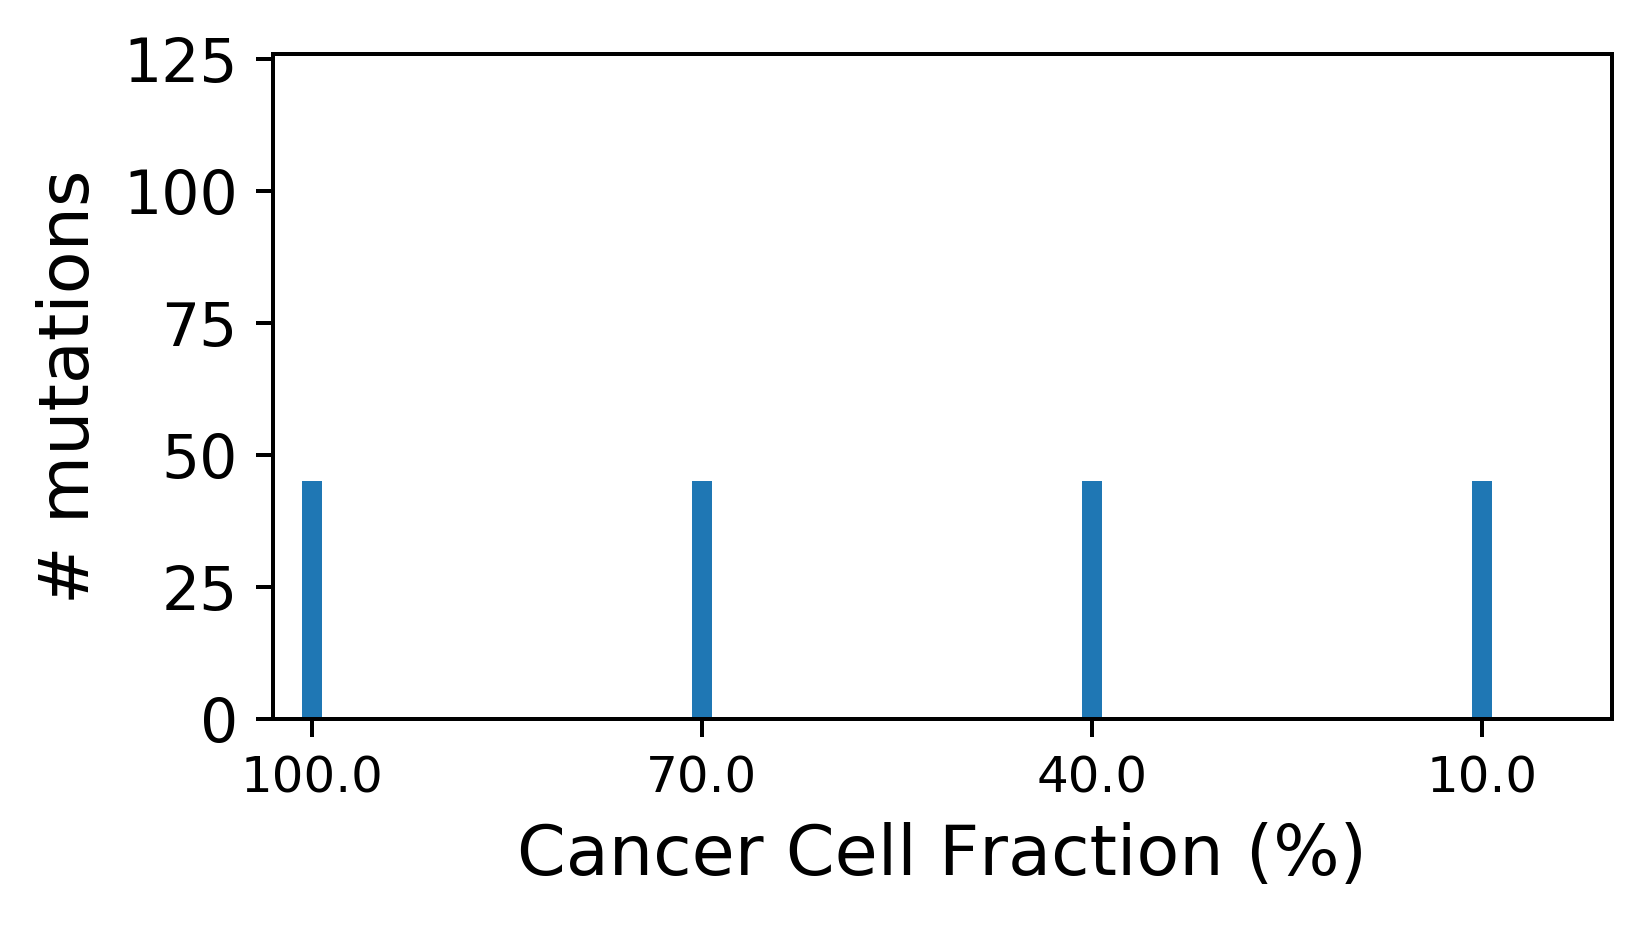
\includegraphics[width = 1.0\linewidth, trim={0 0 0 0}, clip=true]{pyclone_analysis_0_7CN/realcols.png}
		\subcaption{Reference}
		%\label{}	
	\end{subfigure}%
	\hspace{0.01 \linewidth}
	\begin{subfigure}[t]{0.32\linewidth}
		\centering
		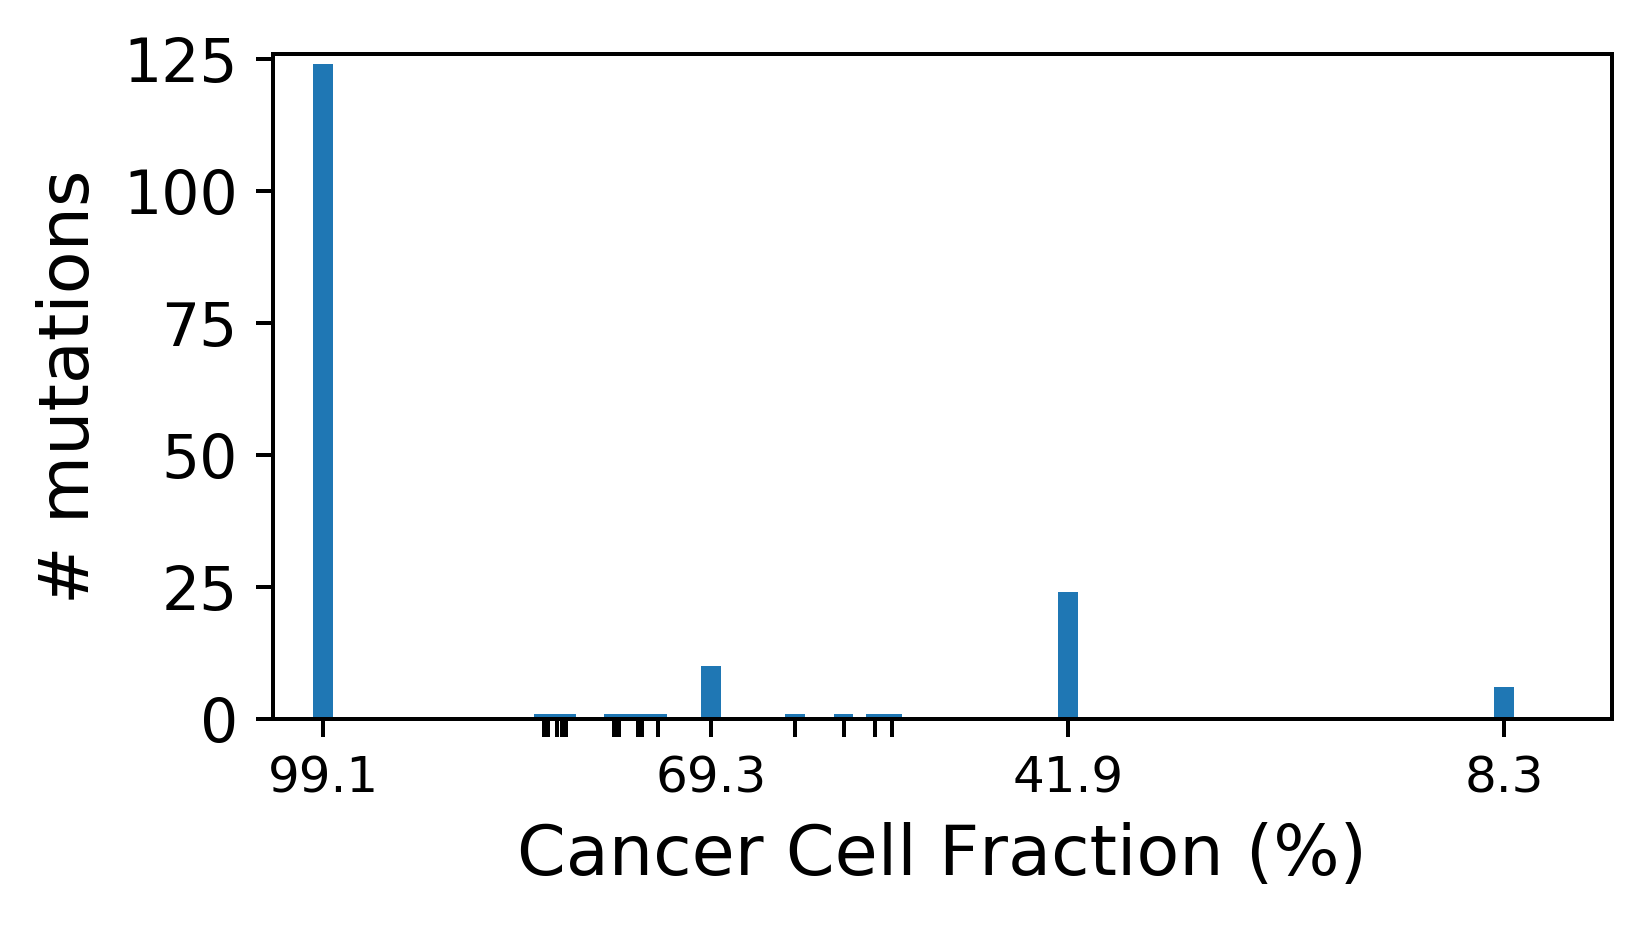
\includegraphics[width = 1.0\linewidth, trim={0 0 0 0}, clip=true]{pyclone_analysis_noCN/cols.png}
		\subcaption{No CNV}	
		%\label{}
	\end{subfigure}%
	\hspace{0.01 \linewidth}
	\begin{subfigure}[t]{0.32\linewidth}
		\centering
		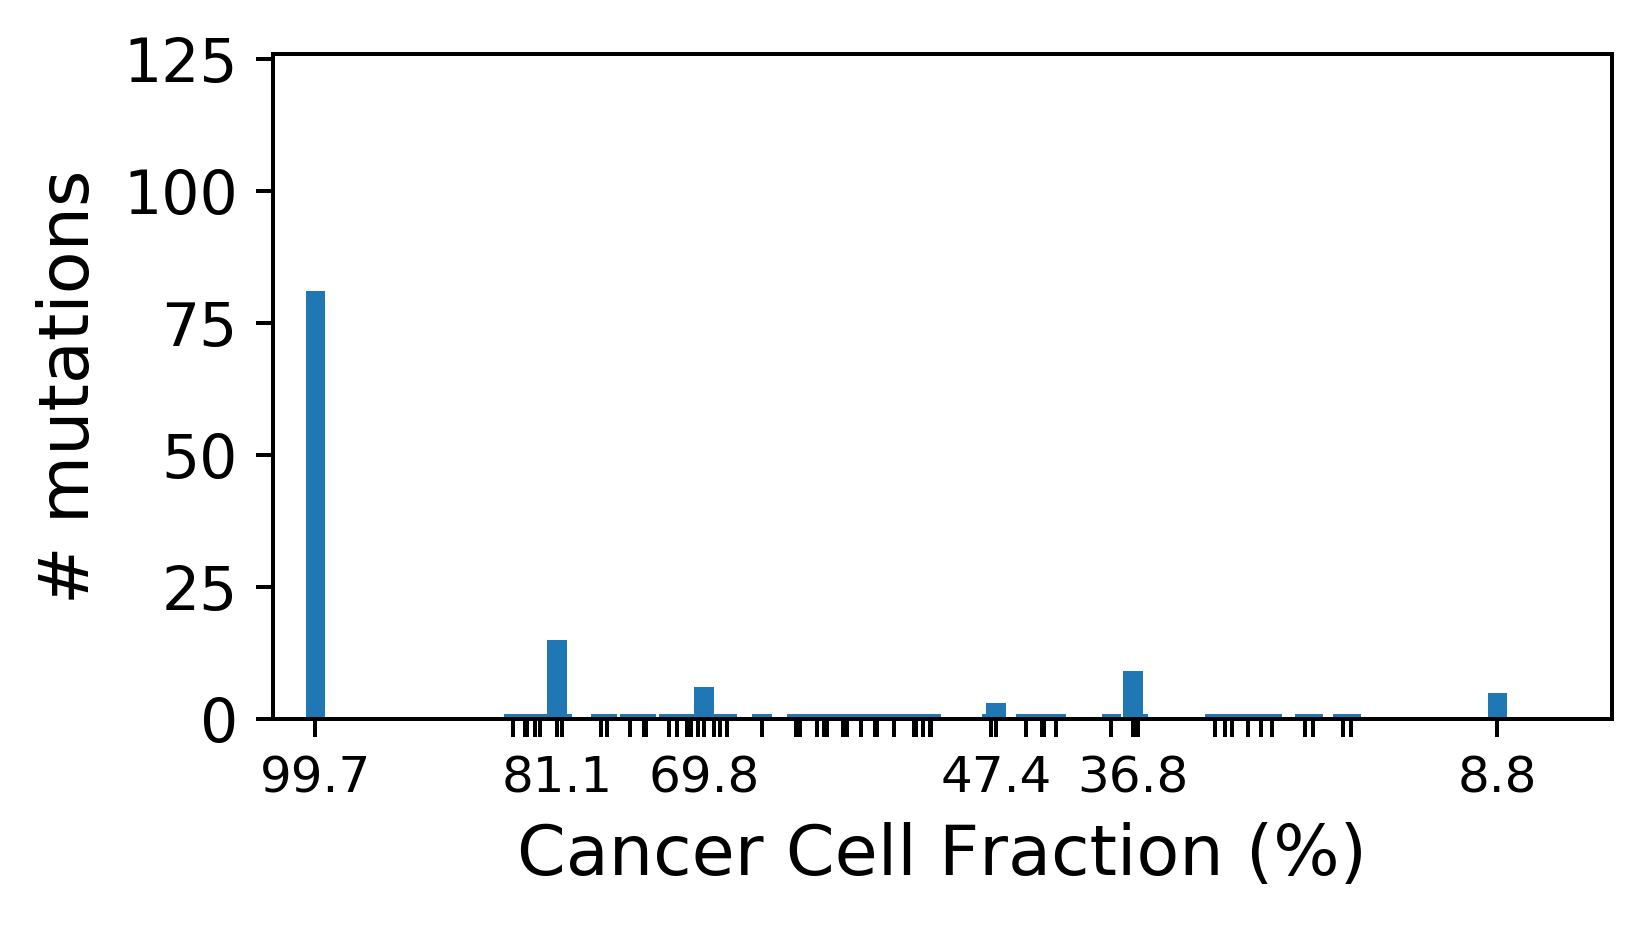
\includegraphics[width = 1.0\linewidth, trim={0 0 0 0}, clip=true]{pyclone_analysis_0_7CN/cols.png}
		\subcaption{70\% CNV}
		%\label{}	
	\end{subfigure}%
\caption{CCF clusters for reference data (a) or PyClone inferences with no copy number variation (b) or copy number alterations at 70\% of sites (c). x-axes indicate CCF of an inferred cluster of mutations, y-axes indicate number of mutations in a cluster. Note that the cluster sizes in (a) are arbitrary and only clusters of more than 1 mutation are annotated in (b), (c).}
\label{fig:pyclone}
\end{figure}

We see that for the data with no copy number variation, PyClone correctly finds four major clusters with cell fractions similar to those of the reference data. In addition, it finds a number of small clusters with only a single mutation. When including copy number variation at 70\% of the sites, PyClone still finds major clusters at approximately 100\%, 70\%, 37\% and 9\%. However, it finds an additional major cluster at 81\% which appears to have erronously been separated from clone A at 100\% CCF. It also finds a small cluster of 2 mutations with a CCF of 47\% which does not exist in the reference data. Performance thus deteriorates significantly both in terms of runtime and accuracy when including copy number variations.

We perform a similar set of analyses using Ccube with numOfClusterPool=1:11 and plot the results in figure \ref{fig:ccube}

\begin{figure}[h]
	\centering
	\begin{subfigure}[t]{0.32\linewidth}
		\centering
		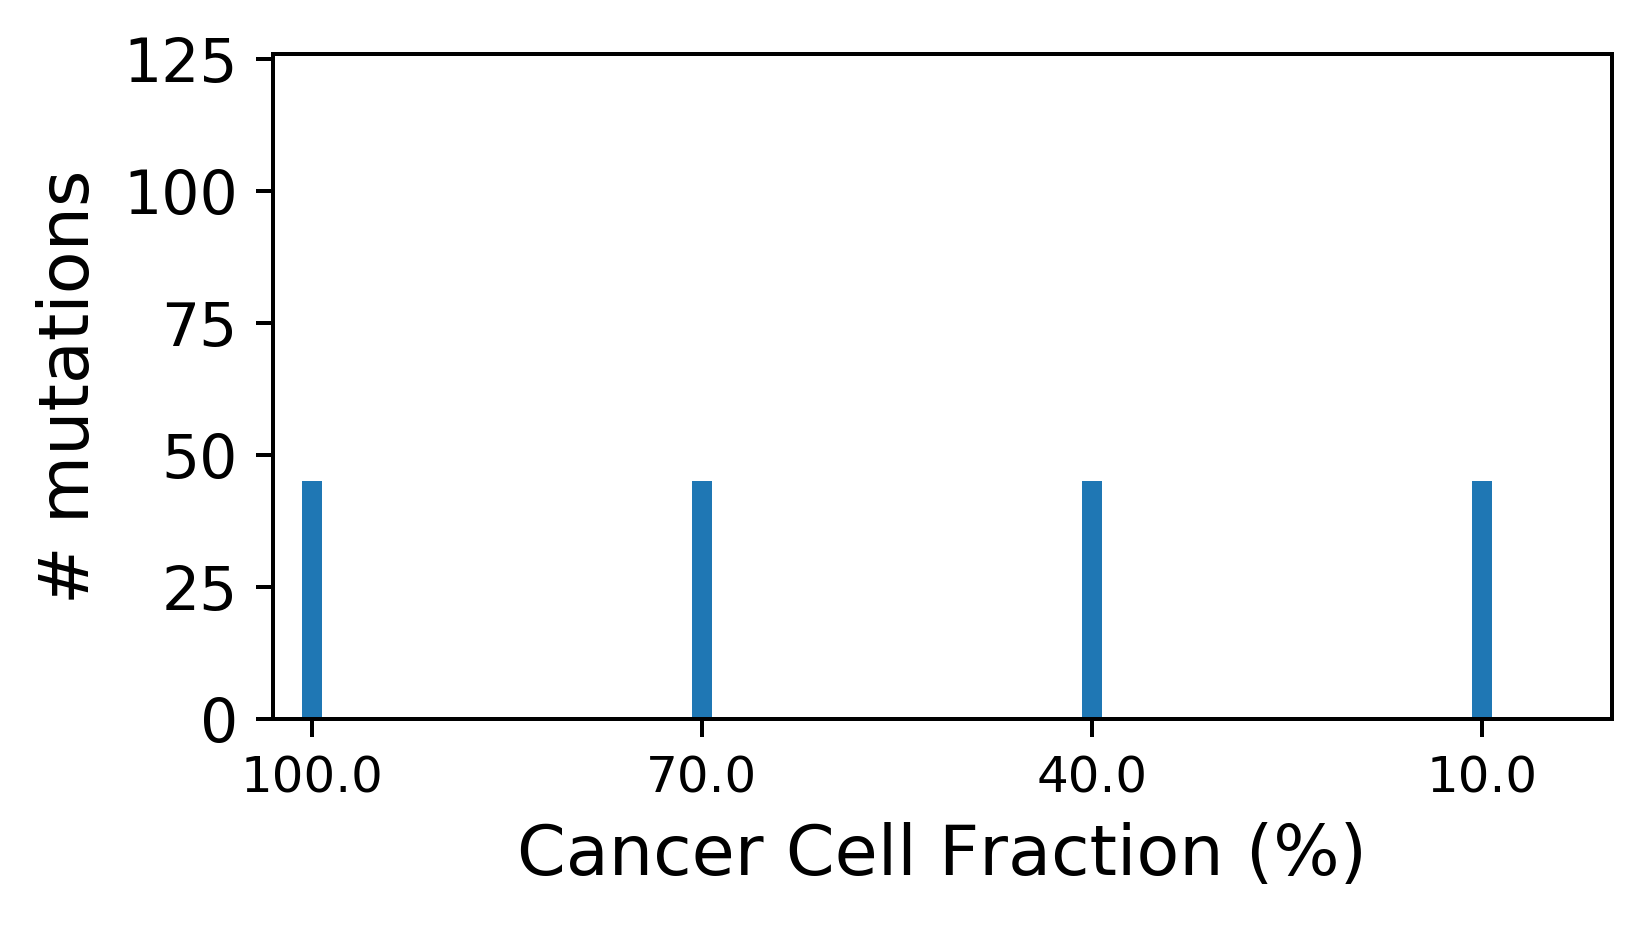
\includegraphics[width = 1.0\linewidth, trim={0 0 0 0}, clip=true]{pyclone_analysis_0_7CN/realcols.png}
		\subcaption{Reference}
		%\label{fig:sim1mul}	
	\end{subfigure}%
	\hspace{0.01 \linewidth}
	\begin{subfigure}[t]{0.32\linewidth}
		\centering
		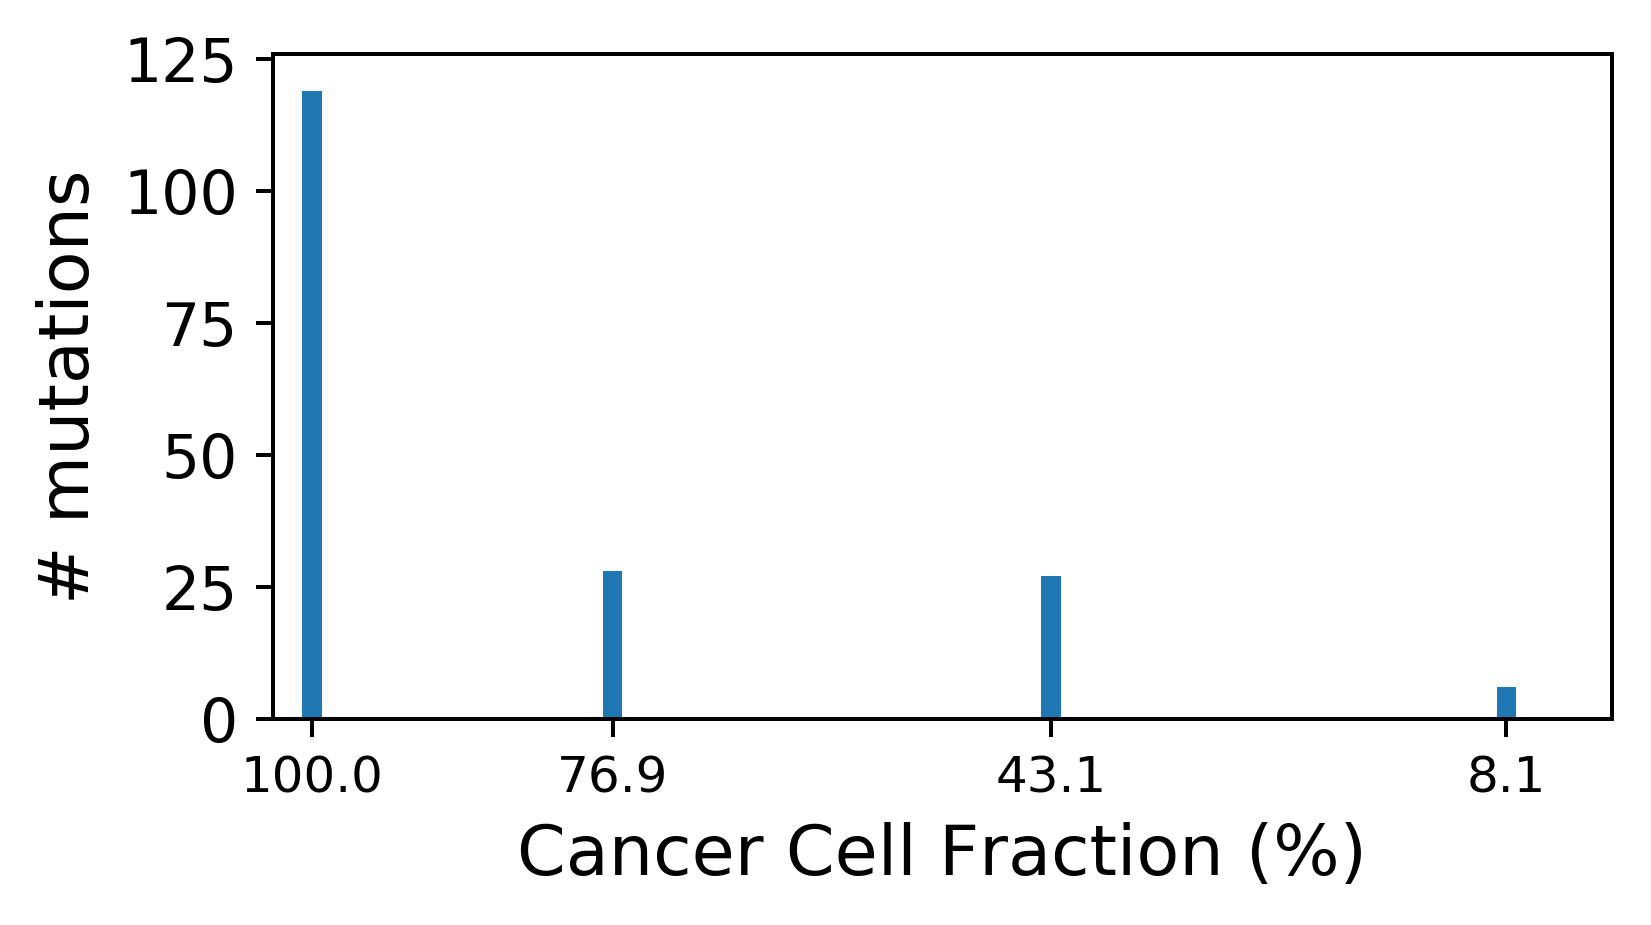
\includegraphics[width = 1.0\linewidth, trim={0 0 0 0}, clip=true]{ccube_analysis_noCN/cols.png}
		\subcaption{No CNV}	
		%\label{}
	\end{subfigure}%
	\hspace{0.01 \linewidth}
	\begin{subfigure}[t]{0.32\linewidth}
		\centering
		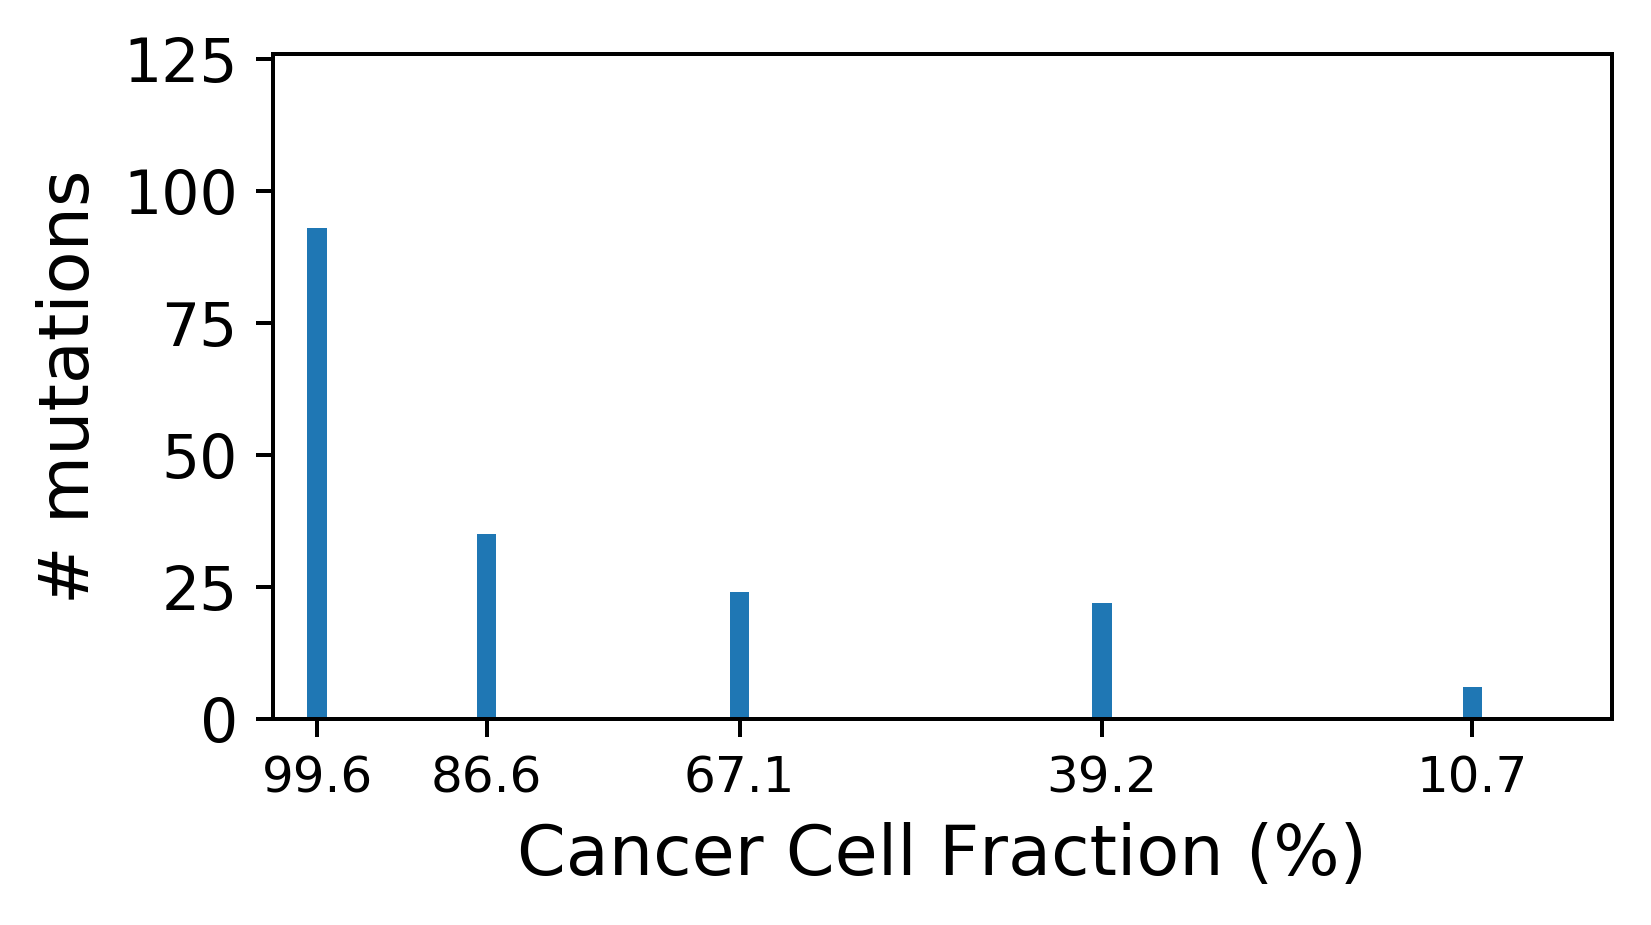
\includegraphics[width = 1.0\linewidth, trim={0 0 0 0}, clip=true]{ccube_analysis_0_7CN/cols.png}
		\subcaption{70\% CNV}
		%\label{fig:sim1mul}	
	\end{subfigure}%
\caption{CCF clusters for reference data (a) or Ccube inferences with no copy number variation (b) or copy number alterations at 70\% of sites (c). x-axes indicate CCF of an inferred cluster of mutations, y-axes indicate number of mutations in a cluster. Note that the cluster sizes in (a) are arbitrary.}
\label{fig:ccube}
\end{figure}

\newpage

We again observe good performance in the case without copy number variations, and in contrast to PyClone Ccube converges to 4 distinct clusters with no singleton noise. However, the CCFs for mutations B and C are somewhat overestimated while that of D is underestimated. In contrast, PyClone yielded more accurate estimates of the underlying cancer cell fractions but less accurate clustering.

Ccube performs relatively well compared to PyClone when including copy number variation, although this method also breaks clone A into two separate clusters similar to PyClone, giving rise to an additional cluster at a cancer cell fraction of 87\%.

\subsection*{4}

We proceed to run a Ccube analysis on downsampled data containing either 100 or 20 sites rather than the original 180 sites. This provides less data for the algorithm and we thus expect worse performance.

In figure \ref{fig:CN0} we compare the performance across the three datasets with no copy number variation. We see that performance is relatively robust with 4 clusters at approximately the same cellular fractions being inferred for both 180 and 100 sites. Only three clusters are identified after downsampling to 20 sites. The relative sizes of the clusters also differ between the three datasets, but this may be due to stochasticity in the subsampling rather than errors in the inference. We also note that the inferred CCFs become less consistent with those of the reference dataset following downsampling.

\begin{figure}[h]
	\centering
	\begin{subfigure}[t]{0.32\linewidth}
		\centering
		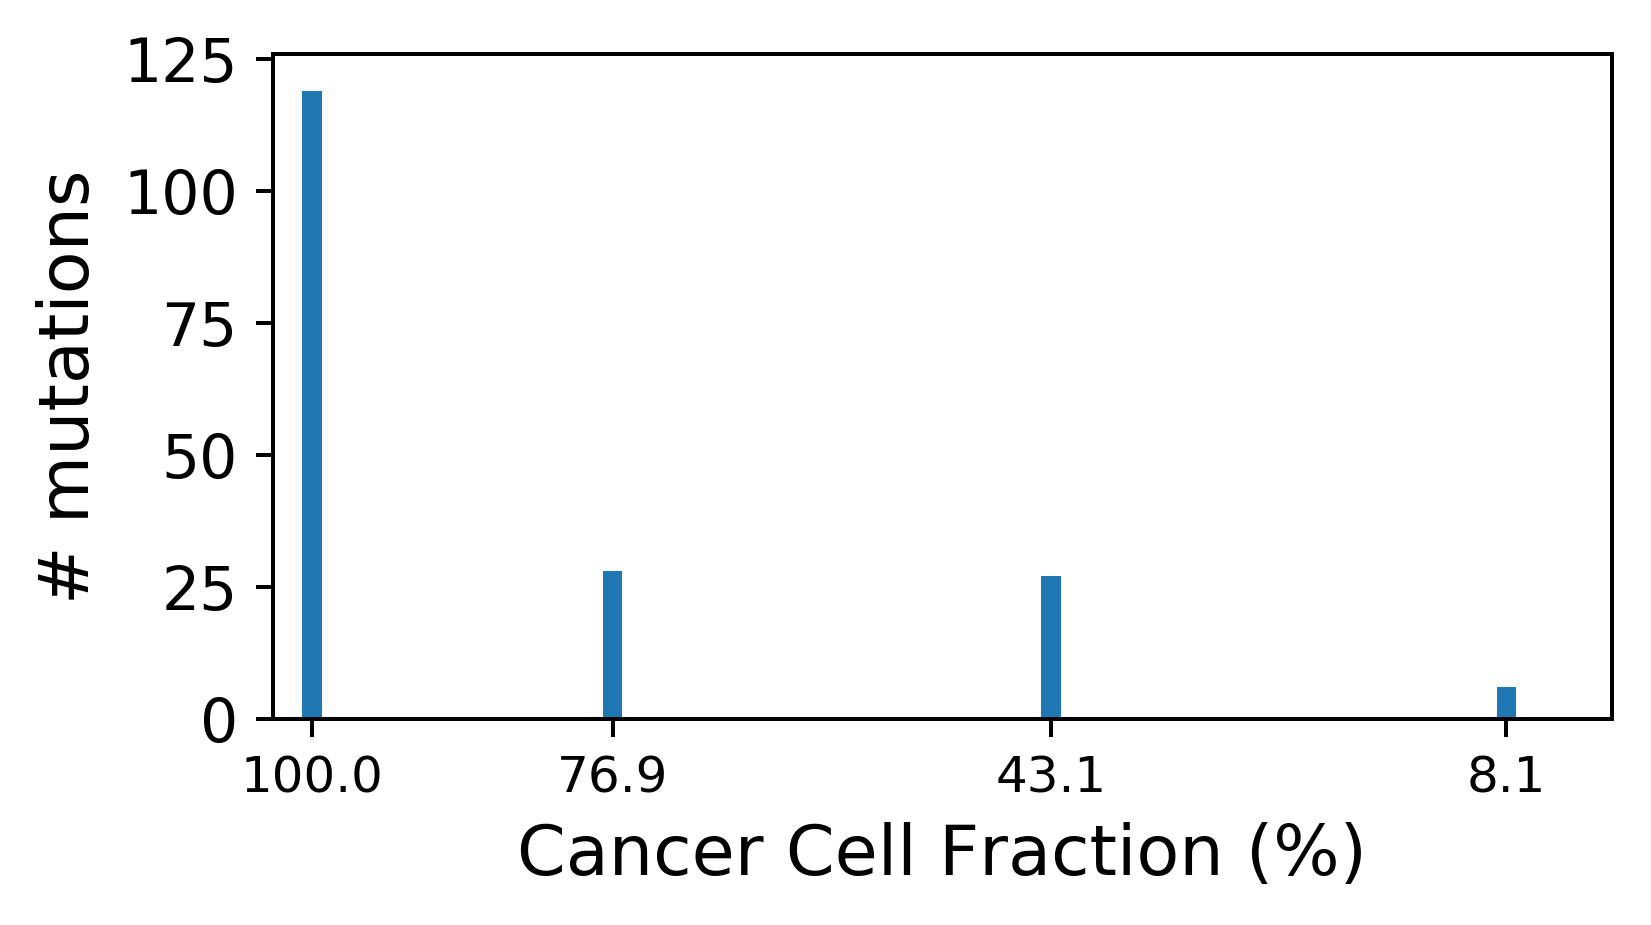
\includegraphics[width = 1.0\linewidth, trim={0 0 0 0}, clip=true]{ccube_analysis_noCN/cols.png}
		\subcaption{180 sites}
		%\label{fig:sim1mul}	
	\end{subfigure}%
	\hspace{0.01 \linewidth}
	\begin{subfigure}[t]{0.32\linewidth}
		\centering
		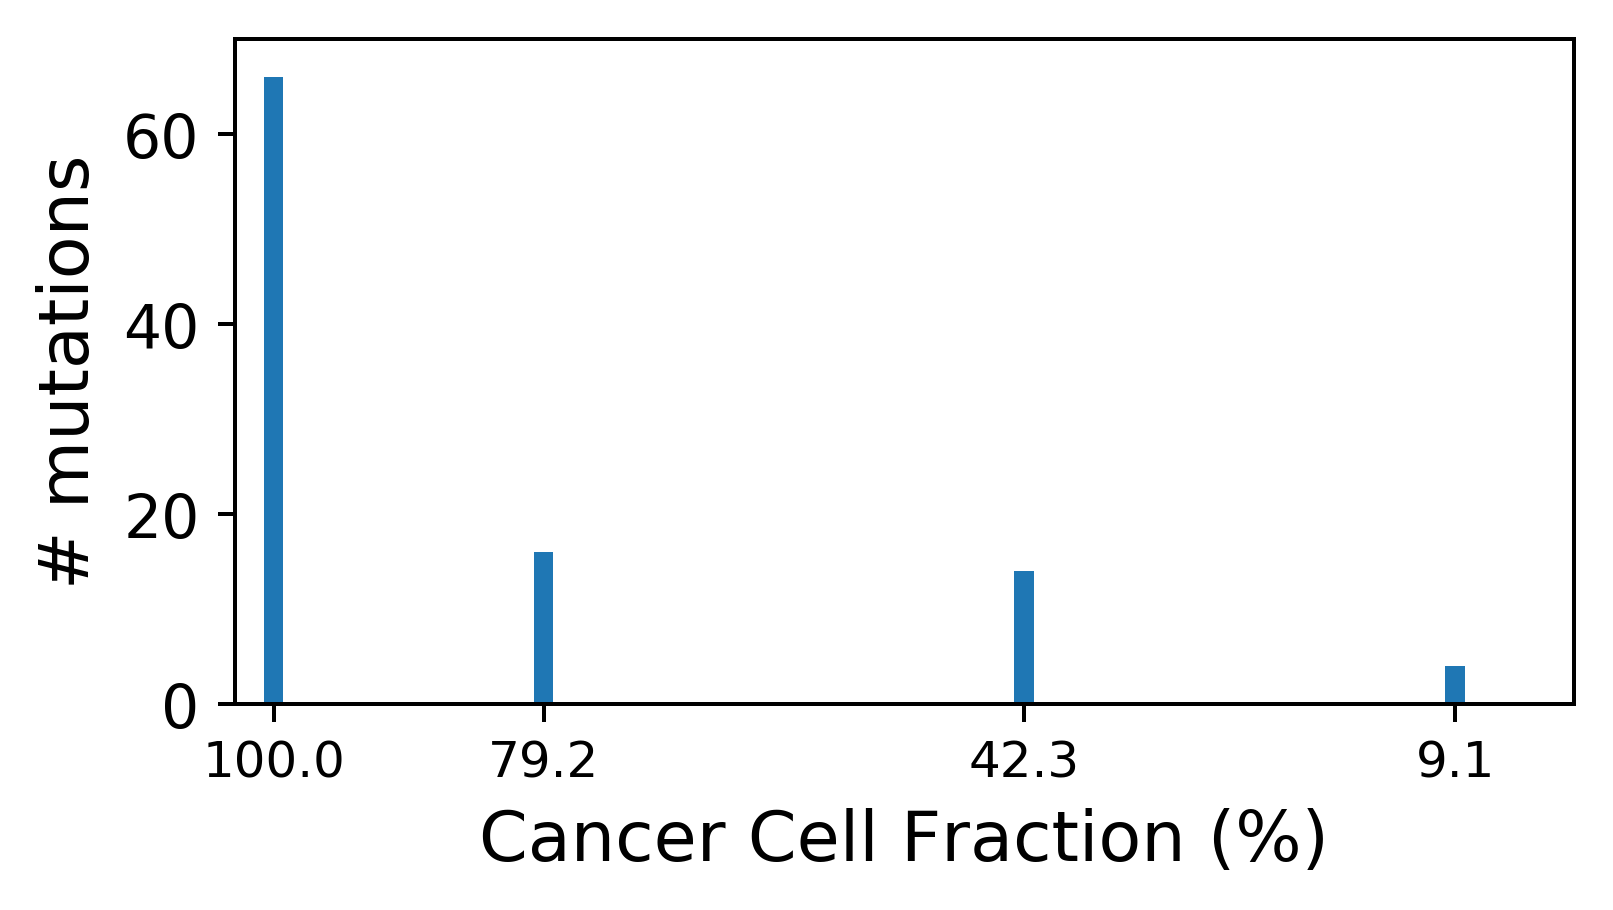
\includegraphics[width = 1.0\linewidth, trim={0 0 0 0}, clip=true]{ccube_analysis_0CN_100/cols.png}
		\subcaption{100 sites}	
		%\label{}
	\end{subfigure}%
	\hspace{0.01 \linewidth}
	\begin{subfigure}[t]{0.32\linewidth}
		\centering
		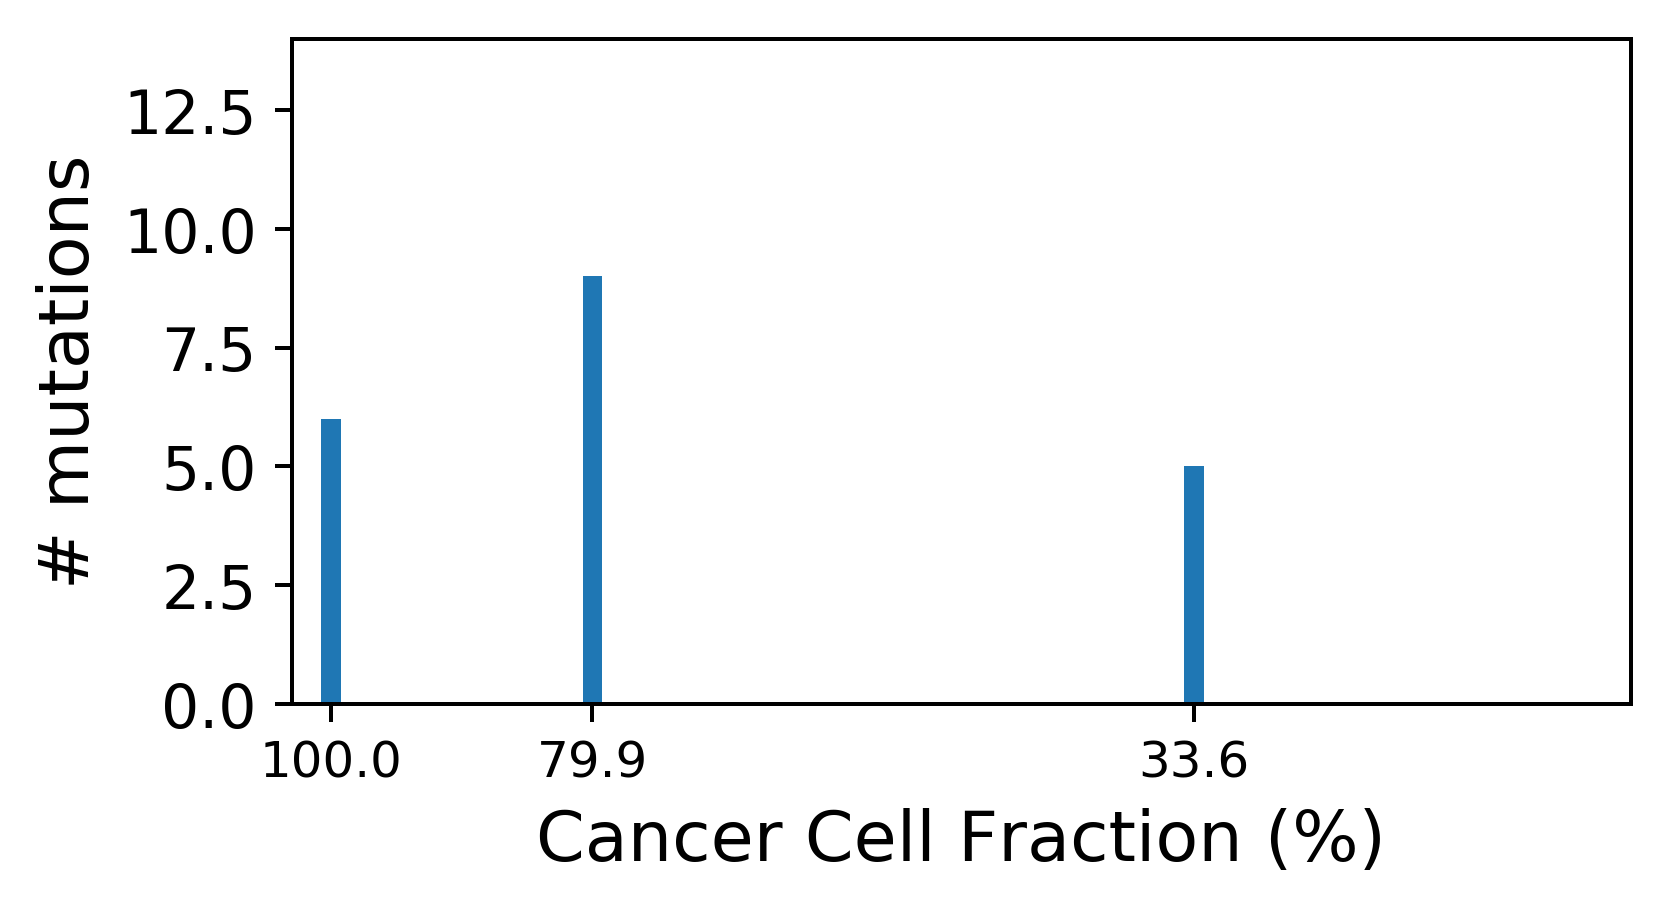
\includegraphics[width = 1.0\linewidth, trim={0 0 0 0}, clip=true]{ccube_analysis_0CN_20/cols.png}
		\subcaption{20 sites}
		%\label{fig:sim1mul}	
	\end{subfigure}%
\caption{CCF clusters inferred by Ccube for the orignal data (a) or downsampled datasets (b,c) in the case of no copy number alterations.}
\label{fig:CN0}
\end{figure}

When considering the dataset with copy number alterations at 70\% of sites, performance is less robust and we again converge to fewer clusters with increased downsampling. These clusters look qualitatively similar to those converged upon after downsampling the data without copy number variation.

\begin{figure}[h]
	\centering
	\begin{subfigure}[t]{0.32\linewidth}
		\centering
		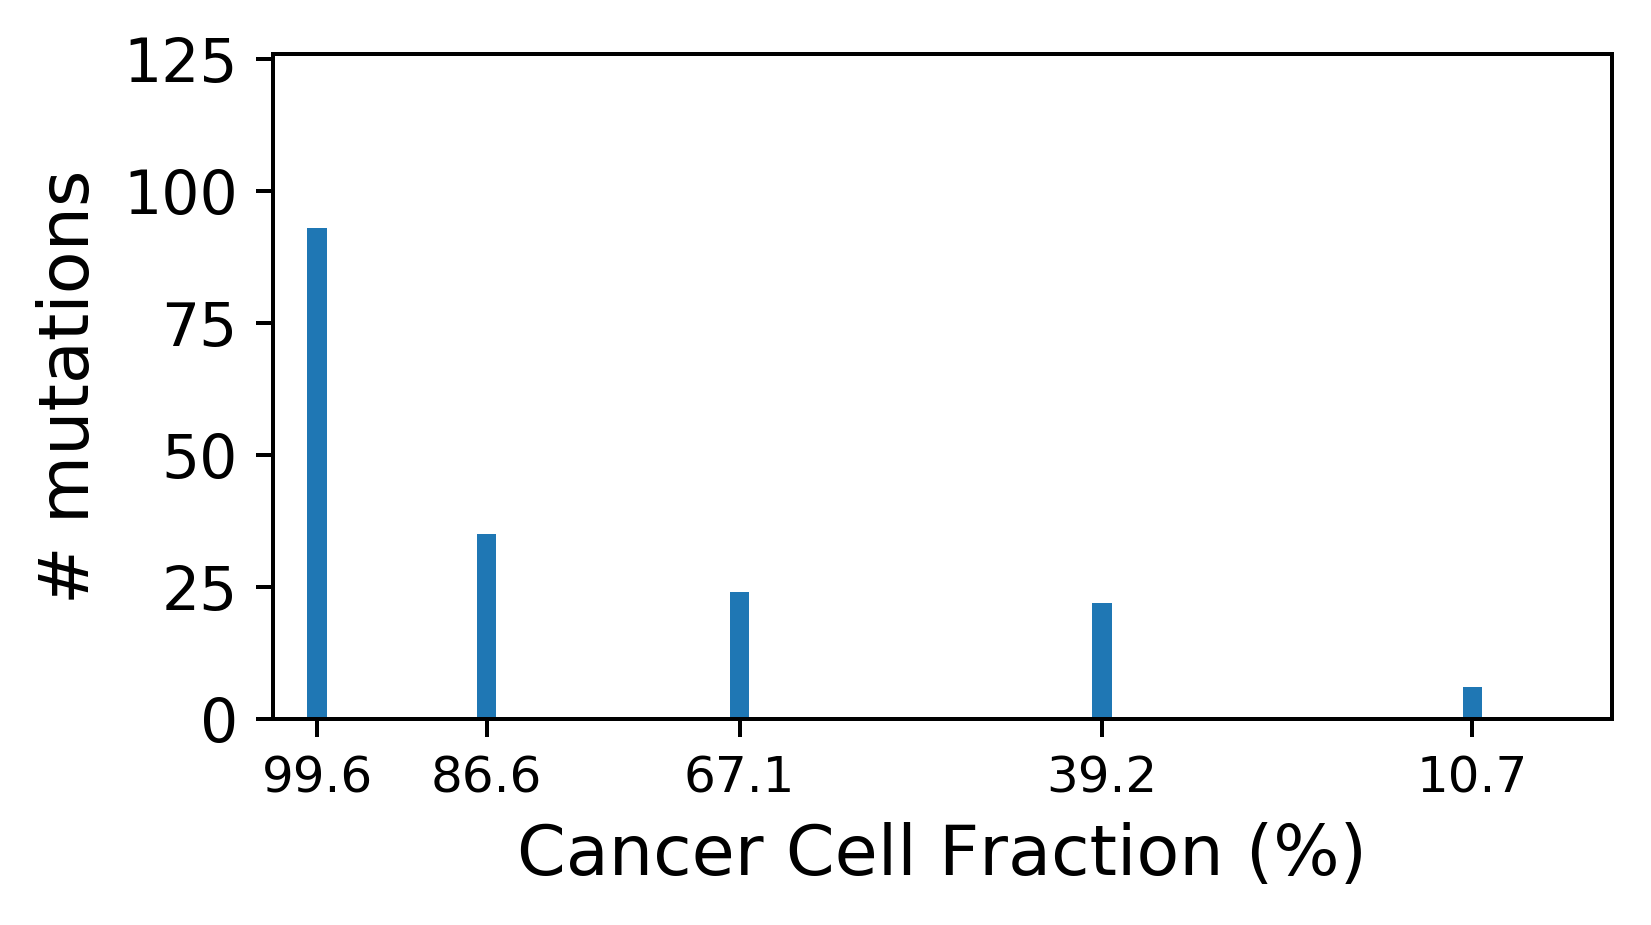
\includegraphics[width = 1.0\linewidth, trim={0 0 0 0}, clip=true]{ccube_analysis_0_7CN/cols.png}
		\subcaption{180 sites}
		%\label{fig:sim1mul}	
	\end{subfigure}%
	\hspace{0.01 \linewidth}
	\begin{subfigure}[t]{0.32\linewidth}
		\centering
		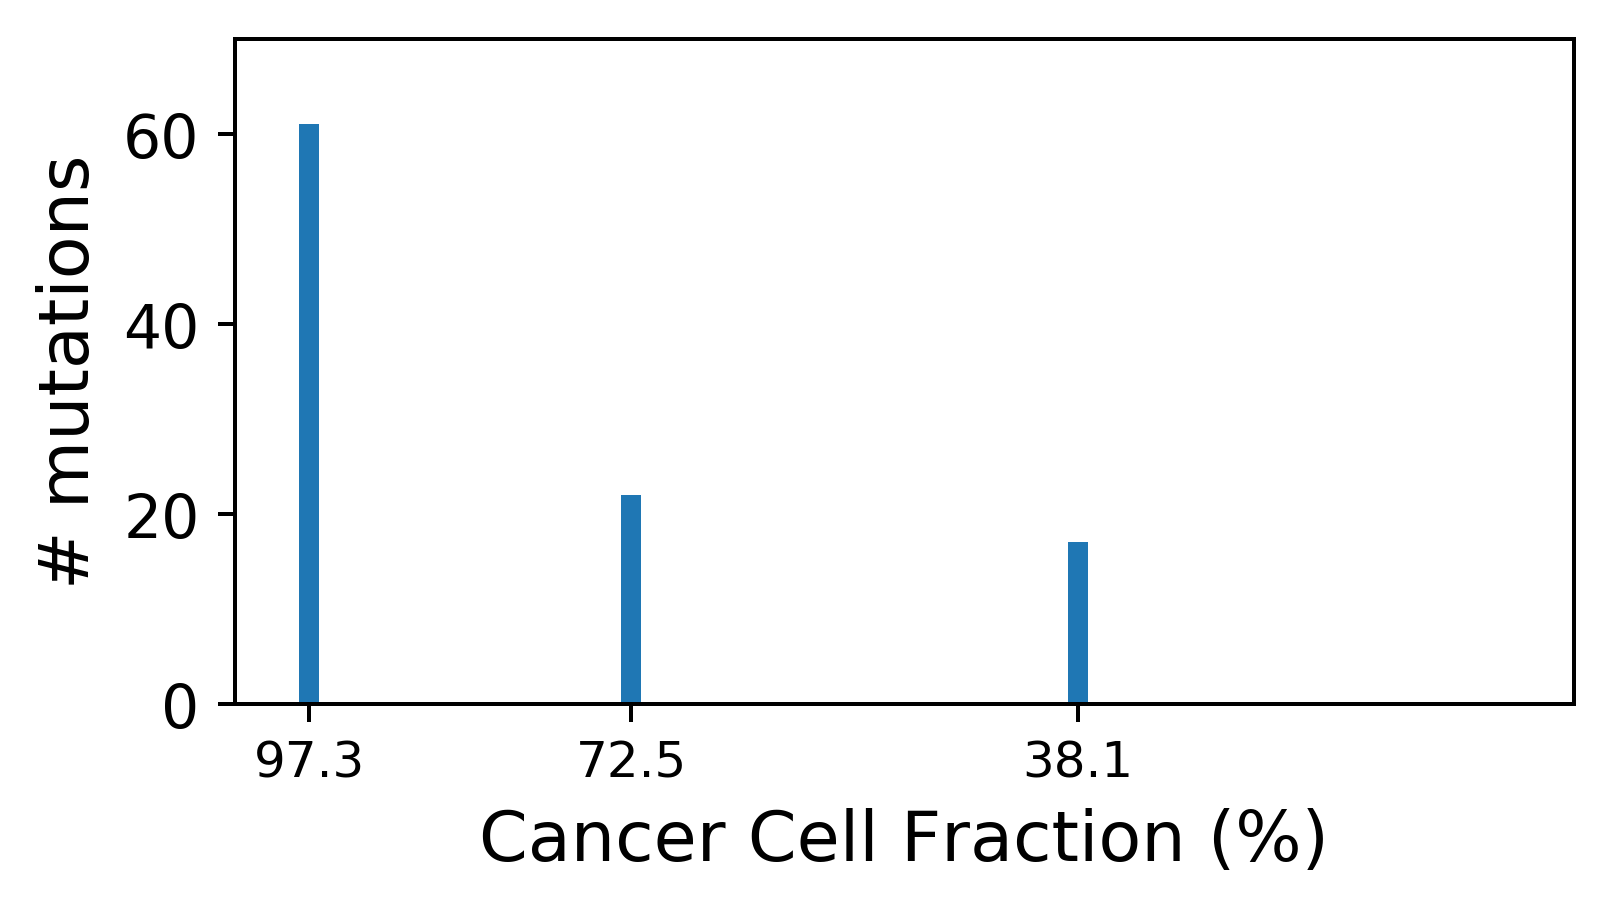
\includegraphics[width = 1.0\linewidth, trim={0 0 0 0}, clip=true]{ccube_analysis_7CN_100/cols.png}
		\subcaption{100 sites}	
		%\label{}
	\end{subfigure}%
	\hspace{0.01 \linewidth}
	\begin{subfigure}[t]{0.32\linewidth}
		\centering
		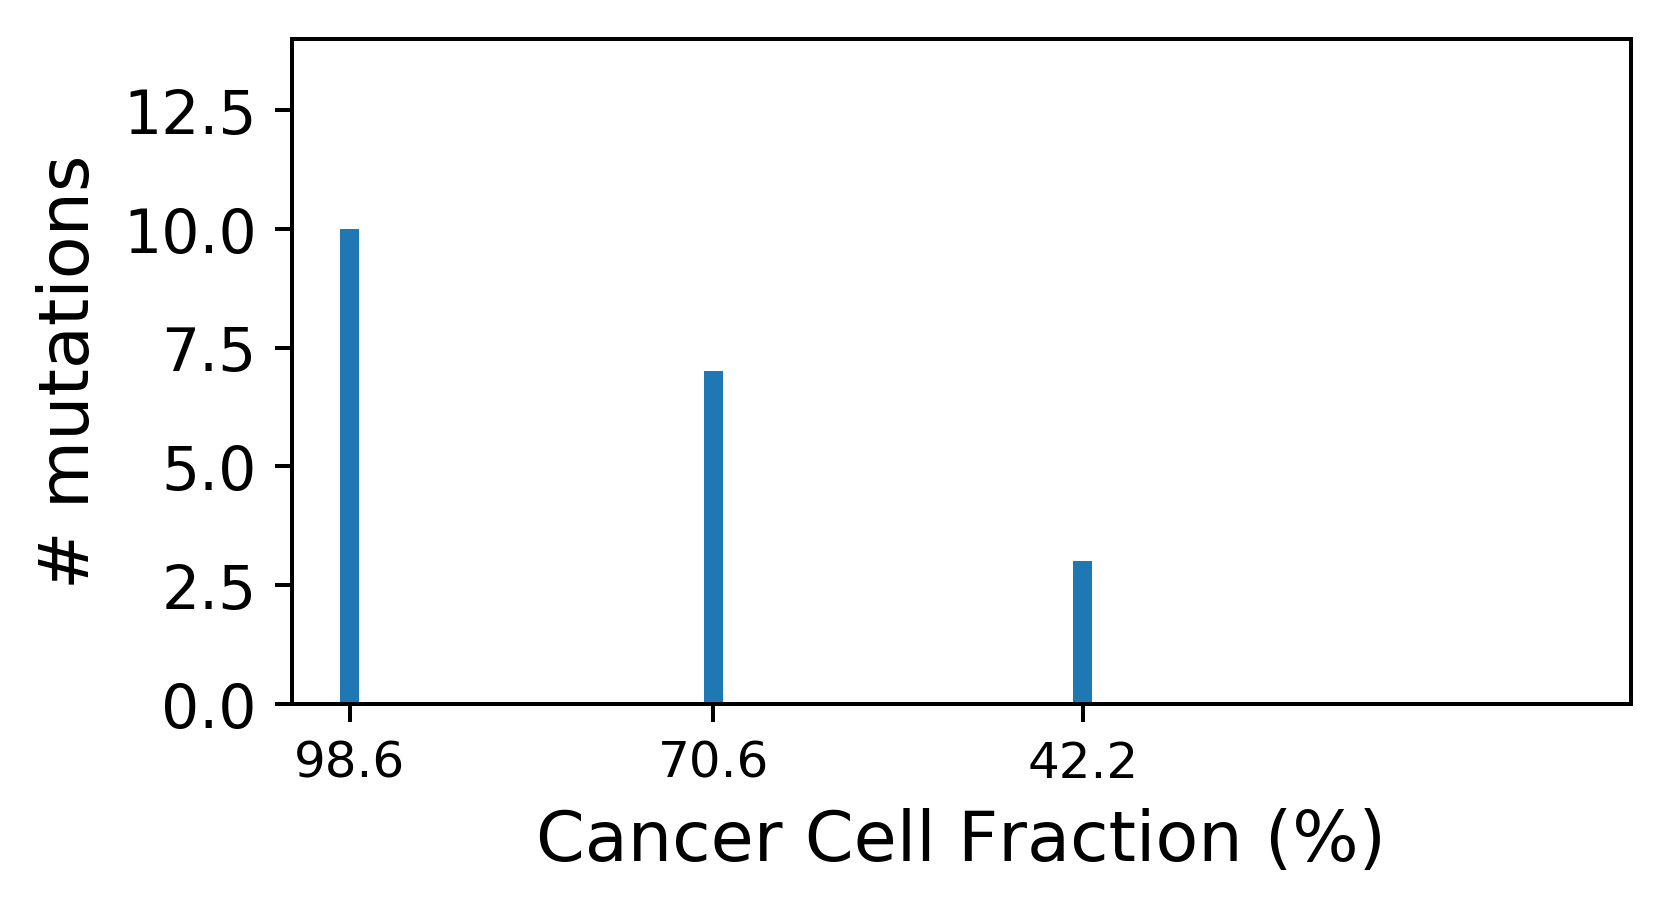
\includegraphics[width = 1.0\linewidth, trim={0 0 0 0}, clip=true]{ccube_analysis_7CN_20/cols.png}
		\subcaption{20 sites}
		%\label{fig:sim1mul}	
	\end{subfigure}%
\caption{CCF clusters inferred by Ccube for the orignal data (a) or downsampled datasets (b,c) with copy number alterations at 70\% of sites.}
\label{fig:CN7}
\end{figure}
\newpage
In summary, we thus conclude that Ccube generally outperforms PyClone both in terms of runtime and clustering. However, when ignoring singleton clusters, the CCFs inferred by PyClone tend to be quite accurate in the absence of copy number variation. We note that in general the problem of clustering becomes substantially harder when copy number alterations are introduced, and that results are less robust with downsampled data.

\subsection*{5}

PyClone and Ccube are conceptually similar by virtue of both being stochastic methods that use infinite mixture modelling to infer cancer cell fractions from read data and copy number data by clustering genomic sites. In both methods, the tumor is considered to consist of three population at each site; a normal population, a tumor reference population, and a tumor variant population.

Both methods also use data generating models that draw VAFs from a distribution over possible mutational scenarios and CCFs, and then draw reads from a binomial distribution of the VAFs and total read counts. The log likelihood of possible CCF clustering scenarios are assessed and the optimum set of clusters returned as the most likely CCF values.

However, despite these underlying similarities there are also theoretical and methodological differences. For example, PyClone uses a uniform prior over different mutational patterns for generating mutational signatures with one of the possible priors being the Parental Copy Number Prior (PCN). The PCN is equivalent to our simulation of VAFs and read data detailed in sections 6 and 7 below. In contrast, Ccube assumes that the total number of alleles in the reference population is always equal to the total number of alleles in the variant population, i.e. that the copy number change is clonal. This allows the authors to derive a linear relationship between CCF and VAF
\begin{equation}
f = w \phi + \epsilon
\end{equation}
\begin{equation}
w = \dfrac{t(m(1-\epsilon)-n_{tot_t}\epsilon)}{(1-t)n_{tot_n}+t n_{tot_t}}
\end{equation}
Where $\phi$ is the CCF, $f$ is the VAF, $\epsilon$ is the sequencing error, $n_{tot}$ are total copy numbers, $t$ is the tumor purity, and $m$ is the number of mutated chromosomal copies.

This in turn allows Ccube to fit its model using an iterative optimization procedure where the posteriors of the CCFs ($\phi$) are optimized and then clustered using a Student-t mixture model. However, this approach requires pre-specification of the numbers of clusters to be considered followed by model selection based on an estimated lower bound of the maximum likelihood (ELBO).

In contrast, PyClone uses a Bayesian non-parametric clustering method which does not require \textit{a-priori} specification of the number of clusters. PyClone then uses a Markov Chain Monte Carlo (MCMC) simulation to estimate a posterior over possible CCFs. At each iteration of the MCMC, new values of $\phi$ are sampled for each mutation and each cluster of mutations using a Dirichlet Process parametized by a Gamma distribution. By default, this MCMC runs for 10,000 iterations to give an accurate posterior, and clustering is then performed based on a posterior similarity matrix quantifying the co-occurrence of each pair of mutations at each point in the MCMC chain.

However, this gives rise to an algorithm that scales as $\mathcal{O}(N^2M)$ where $N$ is the number of mutations and $M$ is the chain length. This in turn is the reason why the PyClone runtime is significantly longer than the Ccube runtime.

PyClone also allows for the incorporation of multiple samples in a single calculation, e.g. from different points in space and time, which can improve the inference. Additionally, PyClone was designed to work with high very coverage data (read depth $> 100x$), and in the original publication some of the example data was sequenced at 5,000x. We thus note that the somewhat poor performance of PyClone above may be mitigated by increased sequencing depth and multiple samples.

Another reason why more noise and singleton groups are observed for PyClone than for Ccube is that Ccube is explicitly designed to merge small clusters and clusters with similar CCF. Thus in Ccube, clusters with less than 1\% of the total number of mutations are removed, and if two clusters differ by less than 10\% CCF they are merged. This means that Ccube cannot  generate more than at most 11 clusters, explaining the upper bound on the number of clusters in our calculations above.

We also note that both methods provide estimates of uncertainty for each mutational site; something we have not considered in the present report. However, it may also be interesting to compare how these uncertainty estimates compare between the two methods.

%Ccube:
%Assumes that the copy number is clonal; nref=nvar=ntot. This is different from the model in PyClone and the model we use to generate data.
%In Cclone, we write down a posterior log likelihood $\log{(b|d,m)} = \sum_i{\log{(b_i|d_i,m_i)}}$ of the observed data for each site  for which we can write down an evidence lower bound (ELBO). The ELBO can then be maximized numerically which removes the need for a long MCMC simulation.
%However, this requires prior specification of the number of clusters with subsequent model selection. The solution with the best ELBO is selected. Clusters with less than 1\% of the mutations are explicitly removed and re-assigned which may explain this difference from PyClone. Clusters with CCFs less than 10\% apart are merged which prevents us from resolving samples with many clusters of similar CCFs.
%Model fitted with variational Baye's approach rather than MCMC simulation.
%
%PyClone:
%Bayesian method for deeply sequenced data (100x+)
%beta-binomial emission densities
%flexible priors
%Bayesian non-parametric clustering; no need to specify groups a-priory!
%multiple samples from single cancer - we're not taking advantage of this
%High read depth ("Mutations called in exomes were deeply sequenced (\~5,000x)")
%Markov-Chain Monte Carlo simulation for 10000 iterations - takes a while.
%Cluster based on posterior similarity matrix (how often mutations co-cluster in posterior distribution)
%Pairwise posterior similarity matrix: scales as O(N\^2 M) where N is number of mutations and M is MCMC chain length
%I.e. generate parameters  probabilitstically, calculate posterior probability and sample from posterior distribution.
%draw prevalence of mutation n across M samples from Dirichlet Process prior.
%We must specify a prior distribution over state vectors (cN, cR, cV) at each position!!! Cn data from elsewhere. PyClone uses uniform prior over a number of different mutational patterns. One of the possible priors is the Parental Copy Number Prior which is equivalent to our simulatino of data below.
%
%Both allow for estimates of uncertainty which we have ignored in the present report.
%Also note that both cluster according to cellular frequencies rather than phylogenetic relationships
%
%The underlying statistichal models are very similar

\section*{B}

\subsection*{6}

As in the lectures, we consider three different scenarios describing how copy number changes and mutations can co-occur at a single locus. In the following, we denote the total number of alleles at locus $i$  by $n$ and the minor allele count $m$. We assume that all CN changes $(n, m)$ happen in a single step. Denoting the number of mutant alleles $n_B$, the three scenarios are
\begin{enumerate}
\item
SNV occurs after CNA; $n_B = 1$

\item
SNV occurs before CNA on the minor copy; $n_B = m$

\item
SNV occurs before CNA on the major copy; $n_B = n-m$

\end{enumerate}

Given $n_B$ and $n$, $m$ for each clone, we can then calculate $n_A$ and the Variant Allele Frequency ($f_B$) 
\begin{equation}
f_B = \dfrac{n_B}{n} = \dfrac{\sum_{k = 0}^K{\pi_k n_{kB}}}{\sum_{k = 0}^K{\pi_k n_{k}}}
\end{equation}

In this section, we assume that all clones carrying an SNV share the same copy number at this locus and that all cancer cells without the SNV also share a potentially different copy number state. Normal cells are assumed to be diploid, and we assume that only one copy number change and one SNV occur at each site. This divides our tumor into three populations at each site. Denoting the allele counts of the total and mutant alleles $c = (n, n_B)$, these are
\begin{enumerate}
\item
normal cells with $c^N = (2,0)$

\item
reference cancer cells with $c^R = (n^R,0)$

\item
variant cancer cells with $c^V = (n^V,n_B)$
\end{enumerate}

Combining these approximations with our three possible scenarios for the emergence of a mutation gives us three possible count vectors for each cell population as specified below:
\begin{enumerate}
\item
SNV occurs after CNA; $c^R = (n, 0)$ \& $c^V = (n, 1)$

\item
SNV occurs before CNA on the minor copy; $c^R = (2, 0)$ \& $c^V = (n, m)$

\item
SNV occurs before CNA on the major copy; $c^R = (2, 0)$ \& $c^V = (n, n-m)$
\end{enumerate}
$c^N = (2,0)$ in all three cases.

In the following, we consider the clonal tree from assignment 1 (figure \ref{fig:ce1tree}) with $\pi_0 = 0.2$. We assume all sites to be independent and thus choose $n_{B}$ independently for each site. 

\begin{figure}[h]
	\centering
	\begin{subfigure}[t]{0.243\linewidth}
		\centering
		\begin{overpic}[width=1.0\textwidth, trim={48 4 48 0}, clip=true]{../ce1/graph.png}
			%\put(14,103){\rotatebox{0}{\color{black}\normalsize Clonal evolution }}

			\put(38,95){\color{black} \large \textit{\textbf{0}}}
			\put(38,78){\color{black} \large \textit{\textbf{A}}}
			\put(38,58){\color{black} \large \textit{\textbf{AB}}}
			\put(38,39){\color{black} \large \textit{\textbf{ABC}}}

			\put(46,27){\color{black} \large \textit{\textbf{ABCD}}}
			\put(20,3){\color{black} \large \textit{\textbf{ABCDH}}}
			\put(49,3){\color{black} \large \textit{\textbf{ABCDG}}}

			\put(-1.5,27){\color{black} \large \textit{\textbf{ABCE}}}
			\put(-7.5,3){\color{black} \large \textit{\textbf{ABCEF}}}
		\end{overpic}
		%\subcaption{}
		%\label{a}
	\end{subfigure}%
\caption{Clonal evolution tree from assignment 1. Nodes are labelled with their clonal frequency and genotypes.}
\label{fig:ce1tree}
\end{figure}
\newpage
In the Ccube vignette, the authors let the major copy number at each site be $n_{major} \in \{1, 2, 3, 4\}$ with probabilities $p = \{0.3, 0.3, 0.2, 0.2\}$ and they let the minor copy number be $n_{minor} \in \{0,1,2\}$ with probabilities $p = \{0.25, 0.5, 0.25\}$. Assuming that Yuan et al. have put some thought into this choice of copy number probabilities and acknowledging the fact that I know little about what would be a better choice, the same parameters have been used in the following.

This allows us to simulate for each of our 40 sites a major, minor and total copy number. This in turn allows us to find $c^N, c^R, \, \& \, c^V$ conditional on the mutational scenario considered. Given these count vectors, we can now calculate the Variant Allele Frequency using equation \ref{eq:vaf}. In the following, we assume the sequencing error rate to be neglible.
\begin{equation}\label{eq:vaf}
f_B = \dfrac{   (1-\pi_0)\tau \cdot n_B   }{   \pi_0 \cdot 2   +   (1-\pi_0)(1-\tau) \cdot n^R   +   (1-\pi_0)\tau \cdot n^V   } 
\end{equation}
 
We use equation \ref{eq:vaf} to calculate VAFs for all 40 loci in each of the three mutational scenarios above after simulating copy numbers as described. We plot the resulting VAFs as a function of Cancer Cell Fraction (CCF) in figure \ref{fig:ccf_vaf}.

\begin{figure}[h]
	\centering
	\begin{subfigure}[t]{0.30\linewidth}
		\centering
		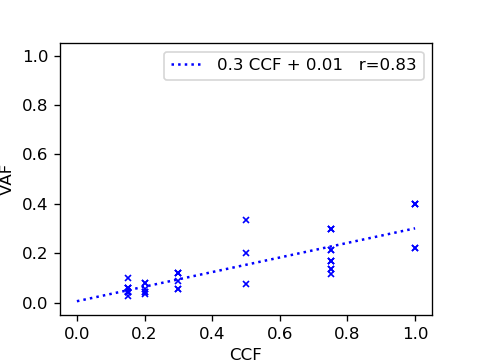
\includegraphics[width = 1.0\linewidth, trim={0 0 20 20}, clip=true]{after_ccf_vaf.png}
		\subcaption{SNV after CNV}
		%\label{fig:sim1mul}	
	\end{subfigure}%
	\hspace{0.02 \linewidth}
	\begin{subfigure}[t]{0.30\linewidth}
		\centering
		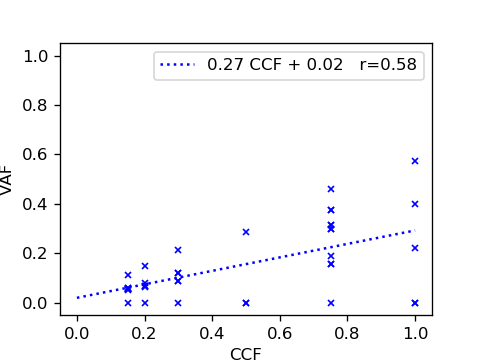
\includegraphics[width = 1.0\linewidth, trim={0 0 20 20}, clip=true]{minor_ccf_vaf.png}
		\subcaption{SNV in minor allele}	
		%\label{}
	\end{subfigure}%
	\hspace{0.02 \linewidth}
	\begin{subfigure}[t]{0.30\linewidth}
		\centering
		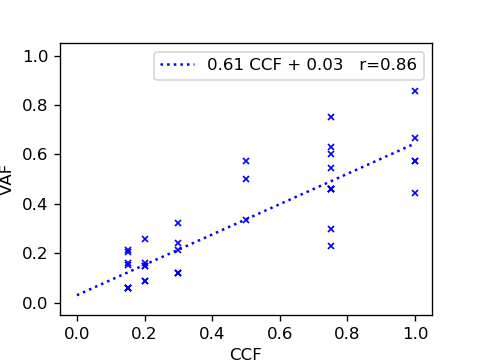
\includegraphics[width = 1.0\linewidth, trim={0 0 20 20}, clip=true]{major_ccf_vaf.png}
		\subcaption{SNV in major allele}
		%\label{fig:sim1mul}	
	\end{subfigure}%
\caption{Variant Allele Frequency as a function of CCF in the three different mutational scenarios discussed in the main text. Dotted lines and legends represent linear lines of best fit.}
\label{fig:ccf_vaf}
\end{figure}

We see that in each case, VAF increases with CCF as expected since variant alleles can only be present in the population that has undergone an SNV, irrespective of major and minor copy numbers. For the the first and third scenario, relations between CCF and VAF are largely linear. We can explain this phenomenon from equation \ref{eq:vaf} by noting that the numerator is linear in $\tau$ and that the $\tau$-dependent terms in the denominator are small when $\tau \rightarrow 0$. At larger $\tau$, the $\tau$-dependent terms cancel when $n^R = n^V$ as in the assumptions underlying the Ccube algorithm and scenario 1 above.

In contrast, there is more noise in the case of SNVs occurring in the minor allele, and much of this arises from cases where the VAF is 0. This is of course an un-realistic scenario as we cannot detect a mutation occurring in an allele that no longer exists which will be discussed further below. In this case, the numerator is 0 and the VAF is no longer linear in CCF.

Finally, we note that we obtain much higher VAFs when mutations occur in the major allele than in either of the other two cases. $n_B$ is always 1 when the SNV occurs after the CNV and $n_B \leq 2$ when the SNV occurs in the minor allele. The weighted average of minor allele frequencies in our model is also equal to 1 which explains why VAF as a function of CCF have similar slopes in the first and second scenarios. In contrast, the mean value of $n_B$ when a mutation occurs in the major allele is 2.3 explaining why the slope in scenario 3 is approximately twice as high.

Finally, we also plot the same data as a bar plot showing the VAF for each individual locus in figure \ref{fig:bylocus} and again note the high degree of variability even for loci with the same CCF, leading to significant VAF overlap between the clusters. This is a major reason why the clustering problem is hard.

\begin{figure}[h]
	\centering
	\begin{subfigure}[t]{0.30\linewidth}
		\centering
		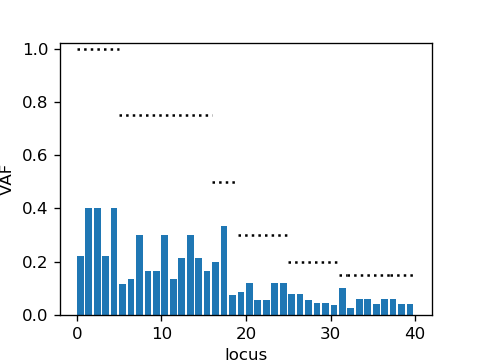
\includegraphics[width = 1.0\linewidth, trim={0 0 20 20}, clip=true]{after_bylocus.png}
		\subcaption{SNV after CNV}
		%\label{fig:sim1mul}	
	\end{subfigure}%
	\hspace{0.02 \linewidth}
	\begin{subfigure}[t]{0.30\linewidth}
		\centering
		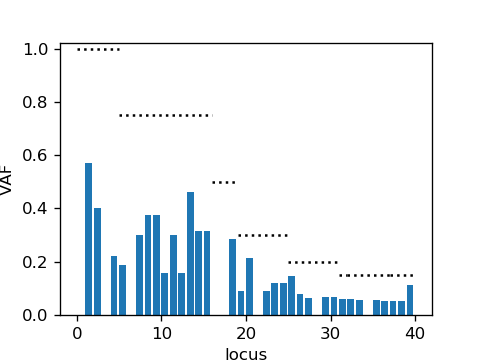
\includegraphics[width = 1.0\linewidth, trim={0 0 20 20}, clip=true]{minor_bylocus.png}
		\subcaption{SNV in minor allele}	
		%\label{}
	\end{subfigure}%
	\hspace{0.02 \linewidth}
	\begin{subfigure}[t]{0.30\linewidth}
		\centering
		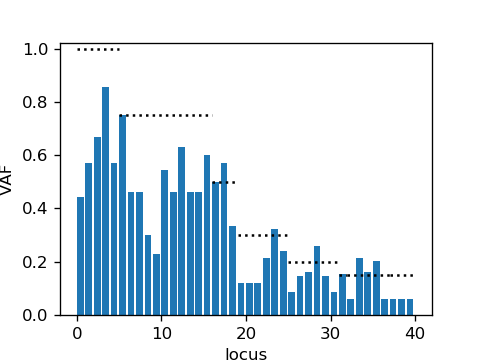
\includegraphics[width = 1.0\linewidth, trim={0 0 20 20}, clip=true]{major_bylocus.png}
		\subcaption{SNV in major allele}
		%\label{fig:sim1mul}	
	\end{subfigure}%
\caption{VAF at each locus of the phylogenetic tree in figure \ref{fig:ce1tree}. Horizontal dotted lines indicate the corresponding CCF at each locus.}
\label{fig:bylocus}
\end{figure}

\subsection*{7}

To simulate real data for analysis by PyClone and Ccube, we use a combination of these three different scenarios since they all occur in vivo. We let it be random whether an SNV occurs before or after the copy number alteration. If the SNV occurs before the CNV and the minor allele count satisfies $m > 0$, we let it be random if the SNV occurred in the major or minor allele. However, if $m = 0$, the SNV must have occurred in the major allele for us to detect it, and we thus let it occur in the major allele with $p=1$. This biases our data towards major allele mutations; an effect that is also expected in real data.

To model read data, we need to take into account the total copy number at each site as the total number of reads at a site $r_i$ is expected to be proportional to the total copy number $n_i$ at that site. Next-generation sequencing data is known to be overdispersed, and we therefore draw the total read count at site i $r_i$ from a negative binomial distribution
\begin{equation}
r_i \sim \text{NegBin}(\lambda_i = 100n_i, s=100) 
\end{equation}
The mean used here is four times higher than that used in the Ccube vignette but still lower than the read-depth used for benchmarking in the original PyClone publication.

Given our read data $r_i$ and VAF $f_{Bi}$ at locus i, we can then draw our variant read count $R_{Bi}$ from a binomial distribution 
\begin{equation}
R_{Bi} \sim \text{Bin}(r_i, f_{Bi})
\end{equation}
Finally we can calculate the reference read count as $R_{Ai} = r_i - R_{Bi}$.

Together with the copy number information from above, this provides all of the data needed to run PyClone and Ccube on our simulated data with the resulting CCF profiles given in figure \ref{fig:sim}. 

\begin{figure}[h]
	\centering
	\begin{subfigure}[t]{0.32\linewidth}
		\centering
		\includegraphics[width = 1.0\linewidth, trim={0 0 0 0}, clip=true]{pyclone_analysis_sim/realcols.png}
		\subcaption{}
		%\label{}	
	\end{subfigure}%
	\hspace{0.01 \linewidth}
	\begin{subfigure}[t]{0.32\linewidth}
		\centering
		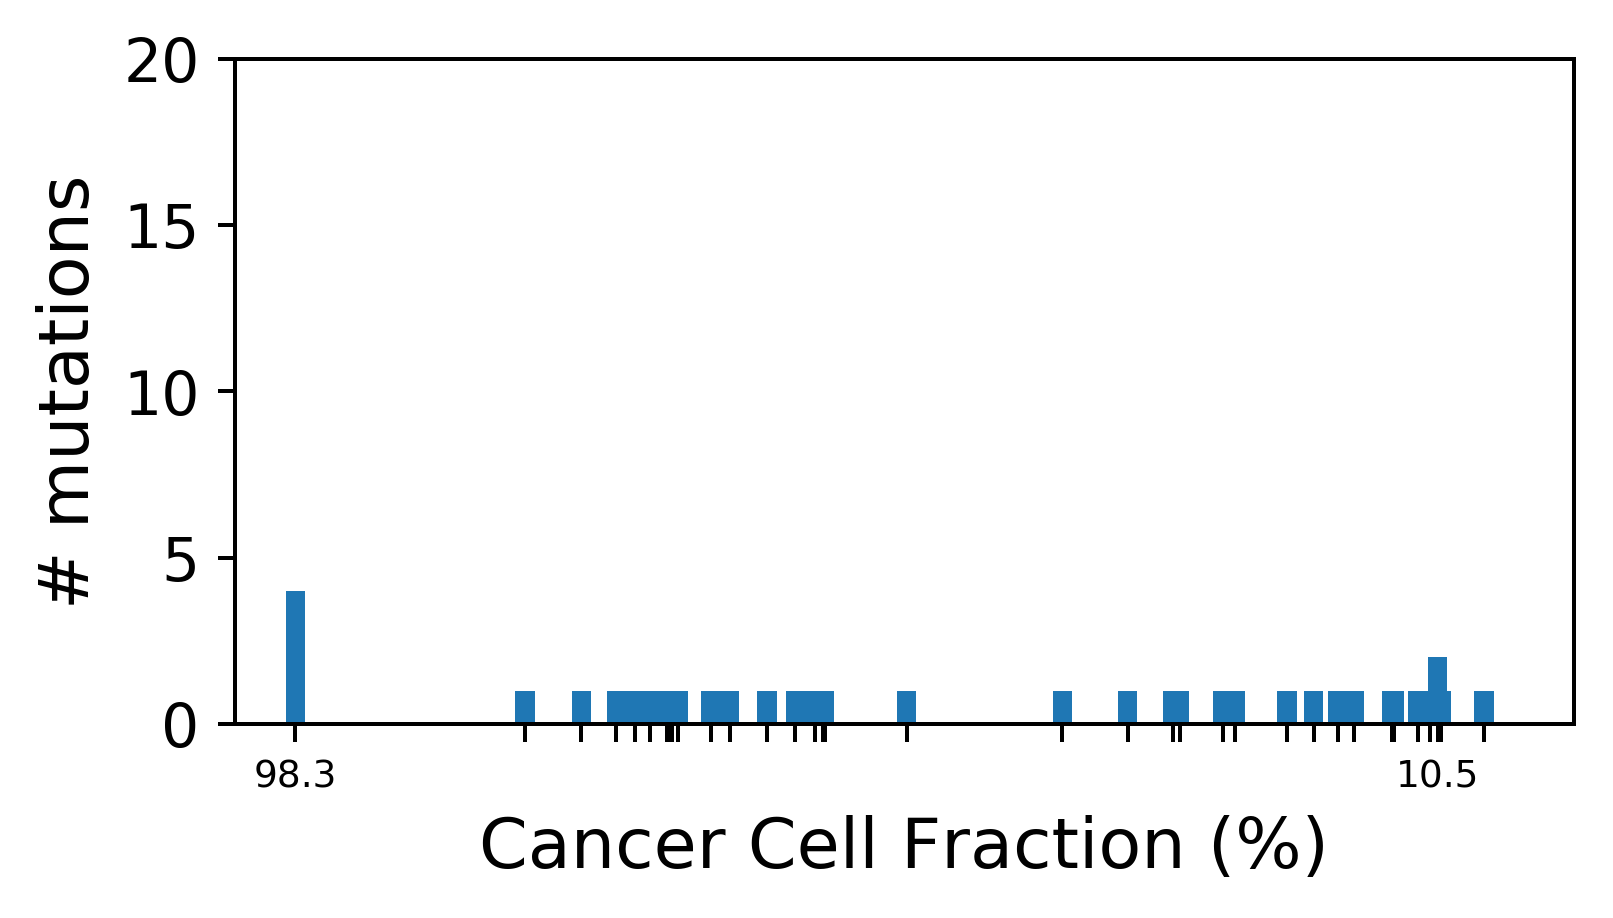
\includegraphics[width = 1.0\linewidth, trim={0 0 0 0}, clip=true]{pyclone_analysis_sim/cols.png}
		\subcaption{}	
		%\label{}
	\end{subfigure}%
	\hspace{0.01 \linewidth}
	\begin{subfigure}[t]{0.32\linewidth}
		\centering
		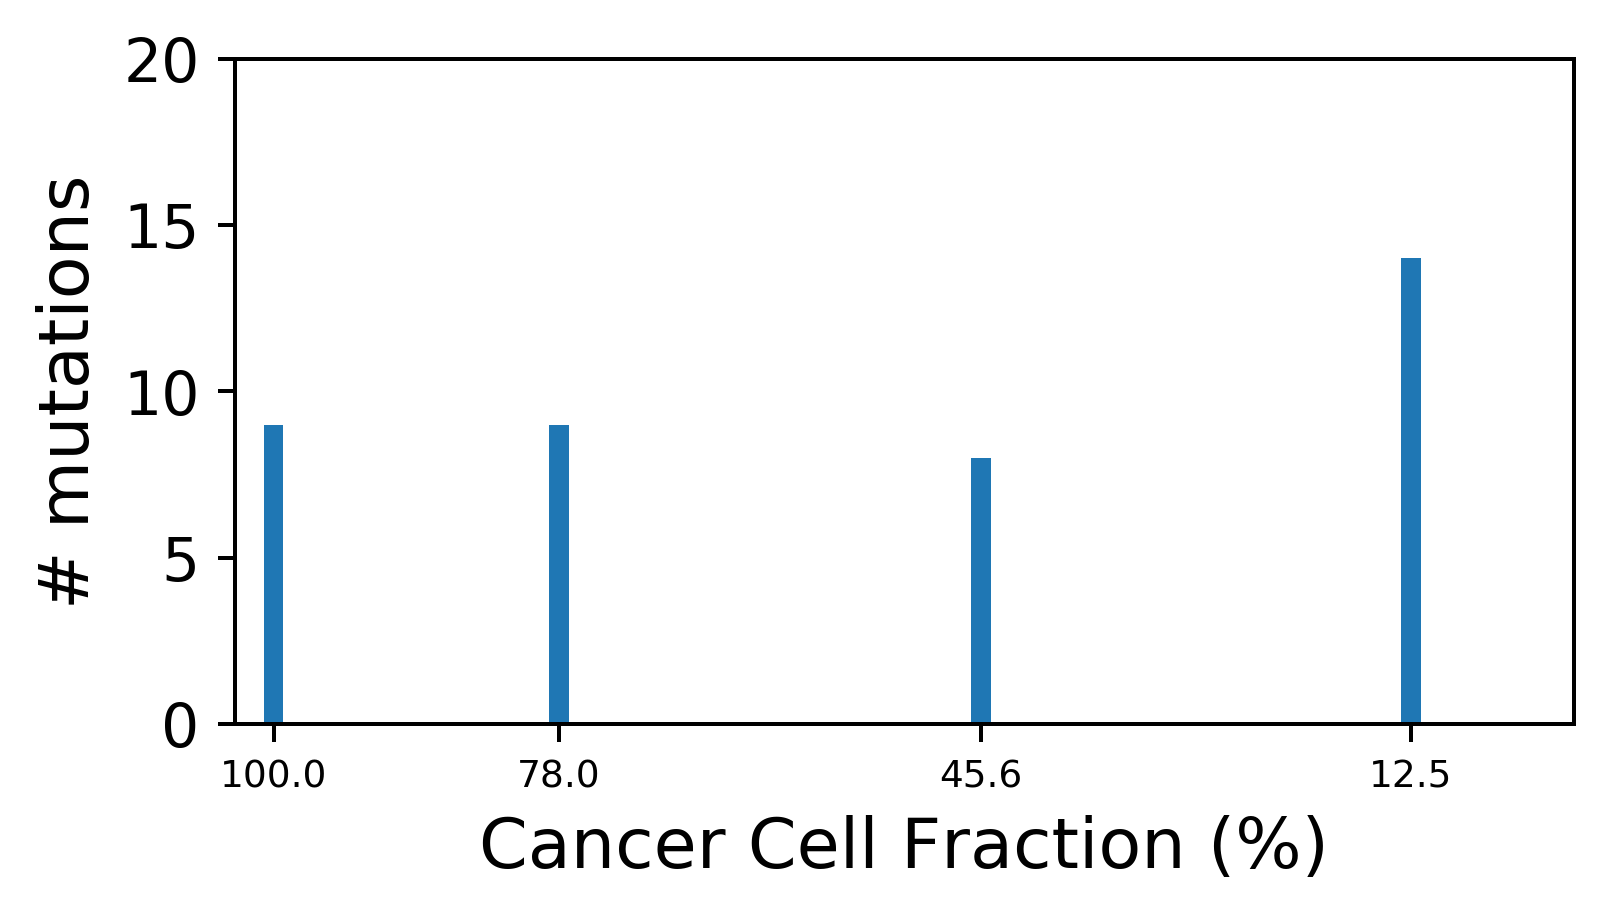
\includegraphics[width = 1.0\linewidth, trim={0 0 0 0}, clip=true]{ccube_analysis_sim/cols.png}
		\subcaption{}
		%\label{}	
	\end{subfigure}%
\caption{(a) CCF clusters for simulated data (100\% CNVs, 100 reads per copy) and the corresponding inferred clusters by PyClone (b) and Ccube (c). x-axes indicate CCFs of the inferred clusters, y-axes indicate number of mutations in a cluster.}
\label{fig:sim}
\end{figure}

\newpage

We see that the performance of both methods is significantly worse than in the example in section A, with Ccube underestimating the number of clusters and PyClone failing to identify more than 1-2 significant clusters.
This drop in performance can be explained by the change in number of sites and number of clusters. In the present dataset, there are too few loci for each clone for PyClone to cluster them accurately, leading to predominantly singleton clusters.

This is similar to our considerations in section 4 where we downsample the original data, but with the clustering problem being even more difficult here since the increased number of clusters leads to more overlap between the distributions of VAFs.
We also note that the data has three clusters at low CCF with very similar CCF values of 15\%, 20\% and 30\%. This leads to merging of clusters in Ccube which by design is unable to resolve clusters separated by less than 10\% CCF.

We find that the task becomes somewhat easier if we have fewer copy number variations, with both algorithms performing better if only 50\% of the sites have simulated copy number changes as illustrated in figure \ref{fig:sim70}. Of course Ccube still fails to resolve the low-CCF clusters; but the three high-CCF clusters are now reasonably accurate.

\begin{figure}[h]
	\centering
	\begin{subfigure}[t]{0.32\linewidth}
		\centering
		\includegraphics[width = 1.0\linewidth, trim={0 0 0 0}, clip=true]{pyclone_analysis_sim50/realcols.png}
		\subcaption{}
		%\label{}	
	\end{subfigure}%
	\hspace{0.01 \linewidth}
	\begin{subfigure}[t]{0.32\linewidth}
		\centering
		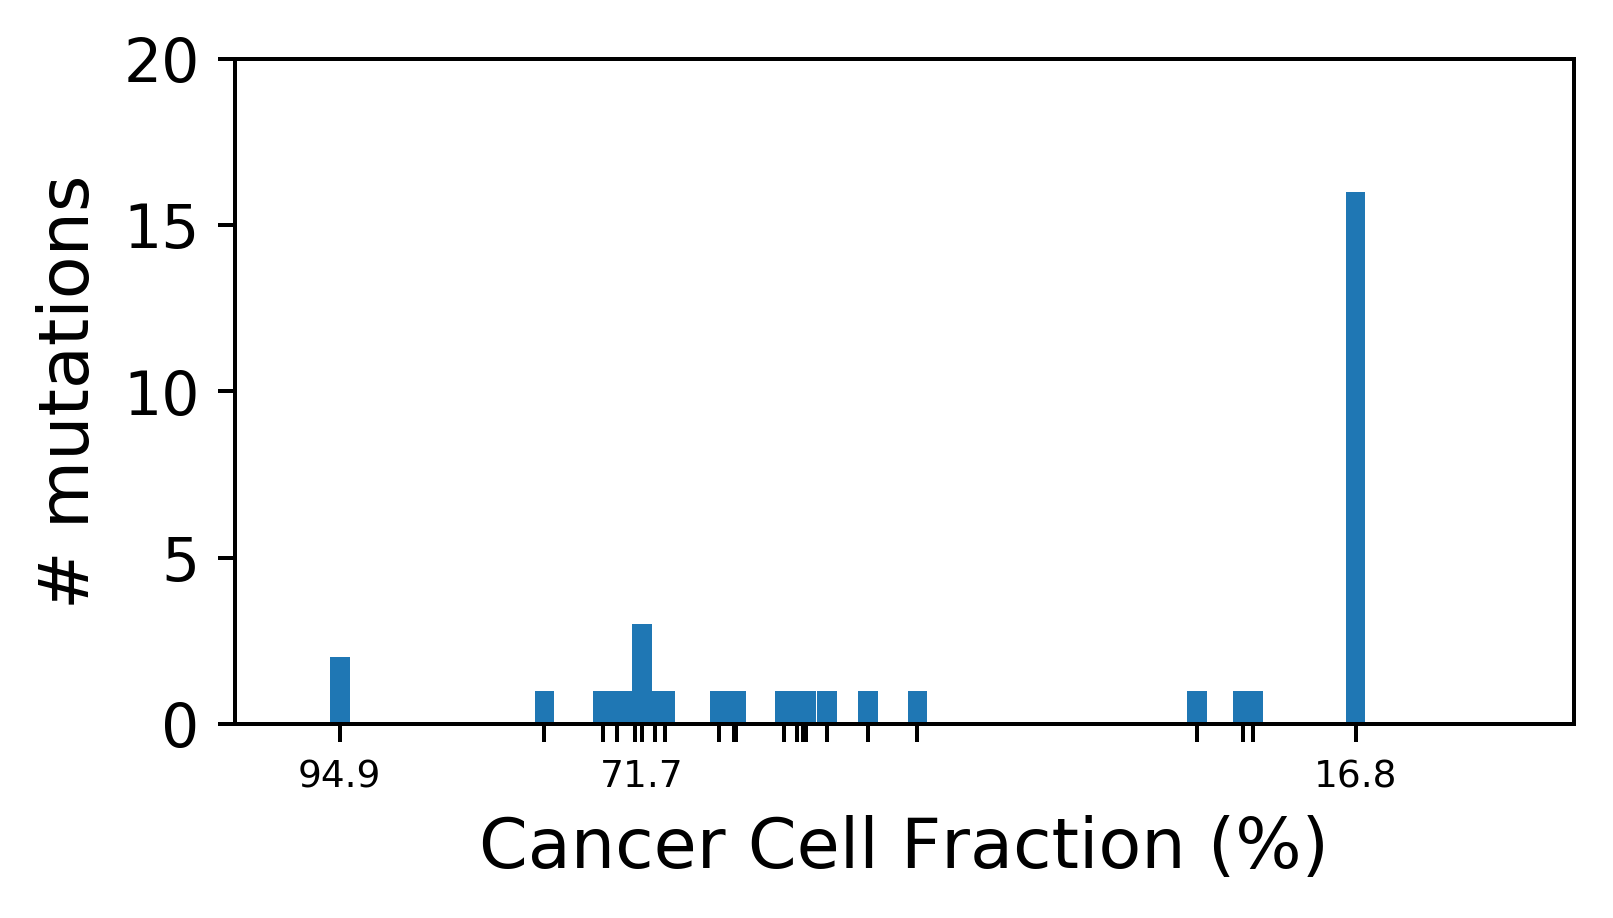
\includegraphics[width = 1.0\linewidth, trim={0 0 0 0}, clip=true]{pyclone_analysis_sim50/cols.png}
		\subcaption{}	
		%\label{}
	\end{subfigure}%
	\hspace{0.01 \linewidth}
	\begin{subfigure}[t]{0.32\linewidth}
		\centering
		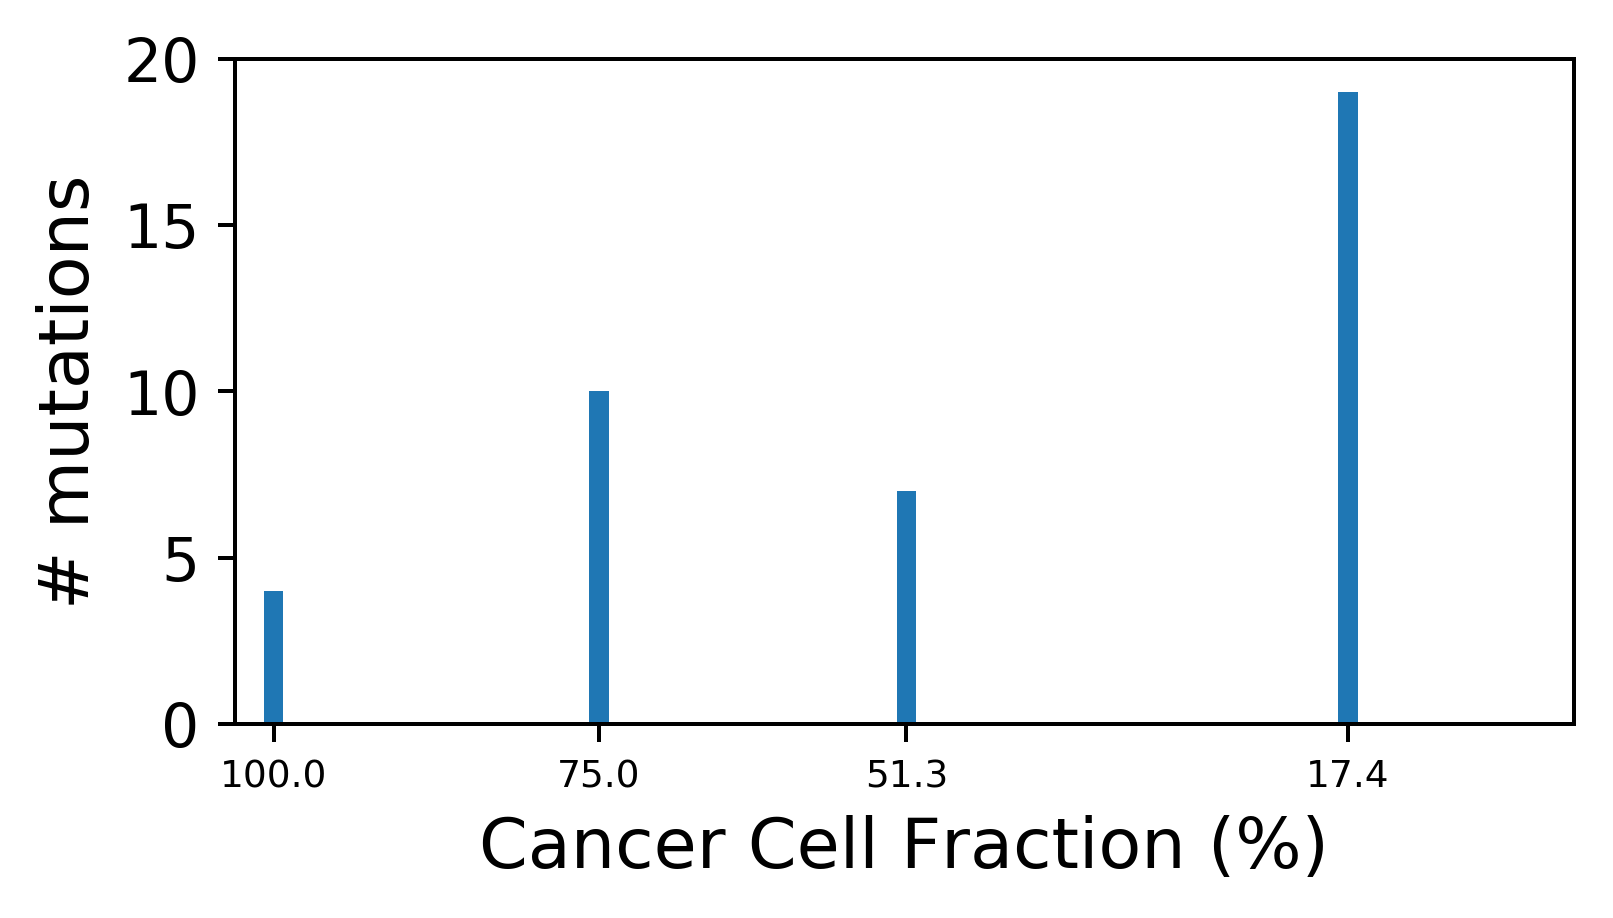
\includegraphics[width = 1.0\linewidth, trim={0 0 0 0}, clip=true]{ccube_analysis_sim50/cols.png}
		\subcaption{}
		%\label{}	
	\end{subfigure}%
\caption{(a) CCF clusters for simulated data (50\% CNVs, 100 reads per copy) and the corresponding inferred clusters by PyClone (b) and Ccube (c).}
\label{fig:sim70}
\end{figure}


Even in the case of 50\% CNV, performance by PyClone is still somewhat poor. However, as expected from section 5, we find that increasing the depth of sequencing by a factor of 10 dramatically increases the performance of PyClone while making less of a difference to Ccube (figure \ref{fig:simdeep}). In fact with a mean read depth of 1000 reads per copy, PyClone correctly identifies all six clusters even with 100\% CNVs, albeit with somewhat erroneous cluster sizes at low CCFs.

\begin{figure}[h]
	\centering
	\begin{subfigure}[t]{0.32\linewidth}
		\centering
		\includegraphics[width = 1.0\linewidth, trim={0 0 0 0}, clip=true]{pyclone_analysis_simdeep/realcols.png}
		\subcaption{}
		%\label{}	
	\end{subfigure}%
	\hspace{0.01 \linewidth}
	\begin{subfigure}[t]{0.32\linewidth}
		\centering
		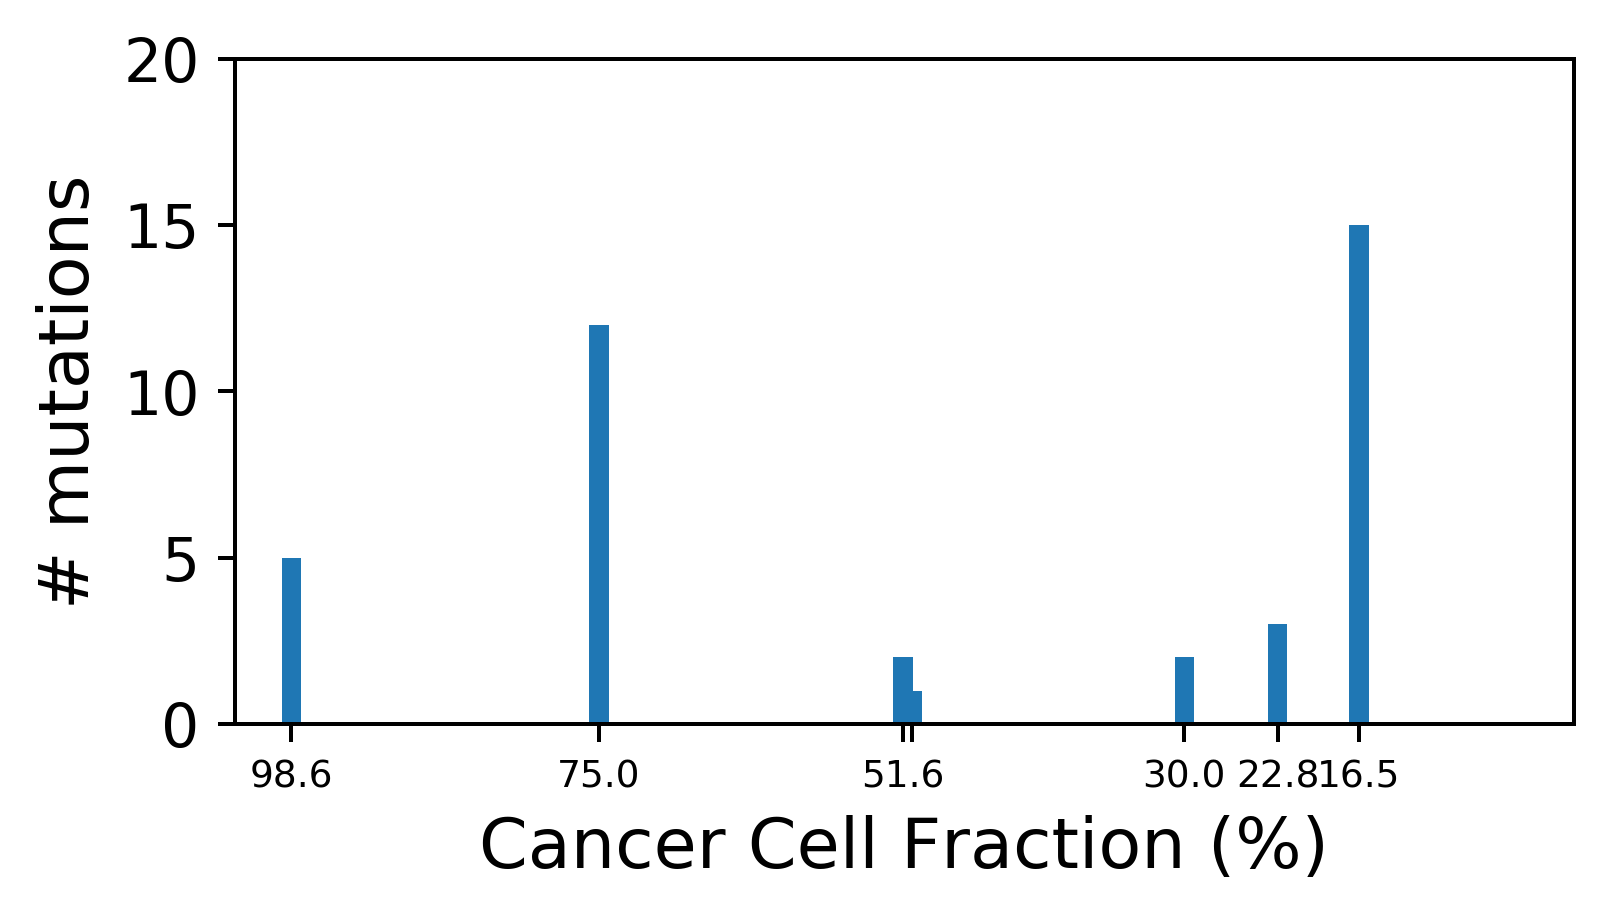
\includegraphics[width = 1.0\linewidth, trim={0 0 0 0}, clip=true]{pyclone_analysis_simdeep/cols.png}
		\subcaption{}	
		%\label{}
	\end{subfigure}%
	\hspace{0.01 \linewidth}
	\begin{subfigure}[t]{0.32\linewidth}
		\centering
		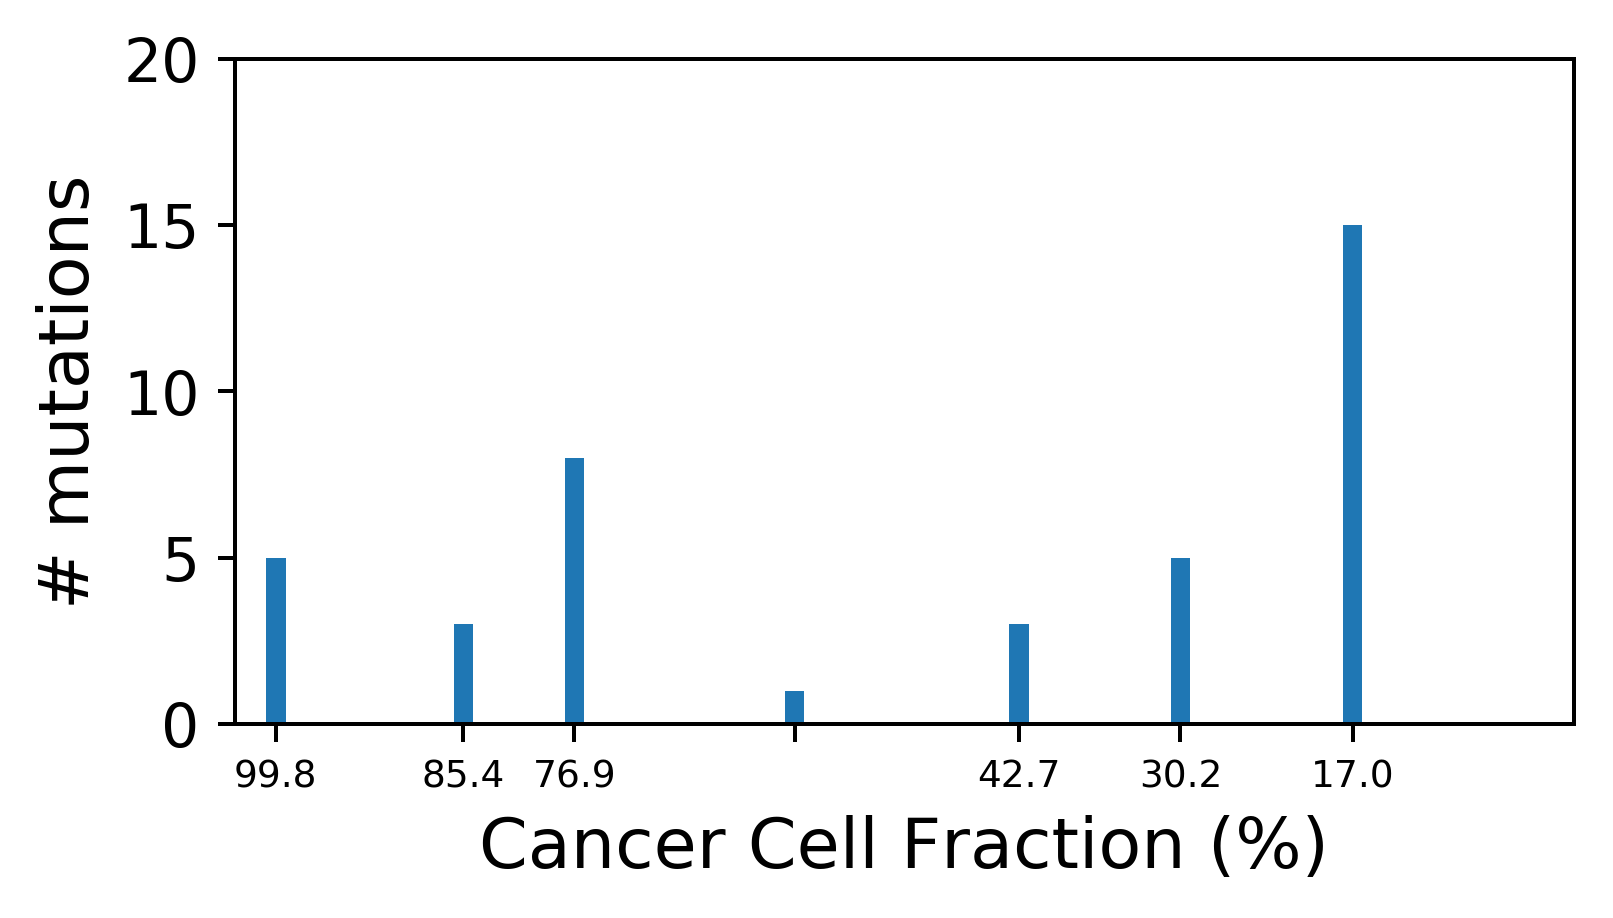
\includegraphics[width = 1.0\linewidth, trim={0 0 0 0}, clip=true]{ccube_analysis_simdeep/cols.png}
		\subcaption{}
		%\label{}	
	\end{subfigure}%
\caption{(a) CCF clusters for simulated data (100\% CNVs, 1000 reads per copy) and the corresponding inferred clusters by PyClone (b) and Ccube (c).}
\label{fig:simdeep}
\end{figure}

\newpage

In summary, it thus seems that Ccube performs substantially better for low-coverage data with few clusters but PyClone appears to be competitive for higher-coverage data with more clusters. PyClone has the additional advantage that no prior cluster number must be specified and that the number of clusters is unbounded. PyClone is also designed for use with multiple samples; a feature we have not leveraged in the present report. We also note that for the present case with only 40 sites, the result of a Ccube analysis differs somewhat when repeating the analysis, but the above figures exemplify the general trends.

We could further investigate the variability and robustness of the methods by generating repeated datasets corresponding to additional samples from the tumors and using more data to infer clusters. However, that is considered beyond the scope of the present report.

\subsection*{8}

We expand our clonal tree from figure \ref{fig:ce1tree} by two metastatic trees in figure \ref{fig:metatree}. One of these is an 'early tree' where the metastatic tumor is seeded from from clone $A$, and the other is a 'late tree' where the tumor is seeded from clone $ABCE$.

\begin{figure}[h]
	\centering
	\begin{subfigure}[t]{0.60\linewidth}
		\centering
		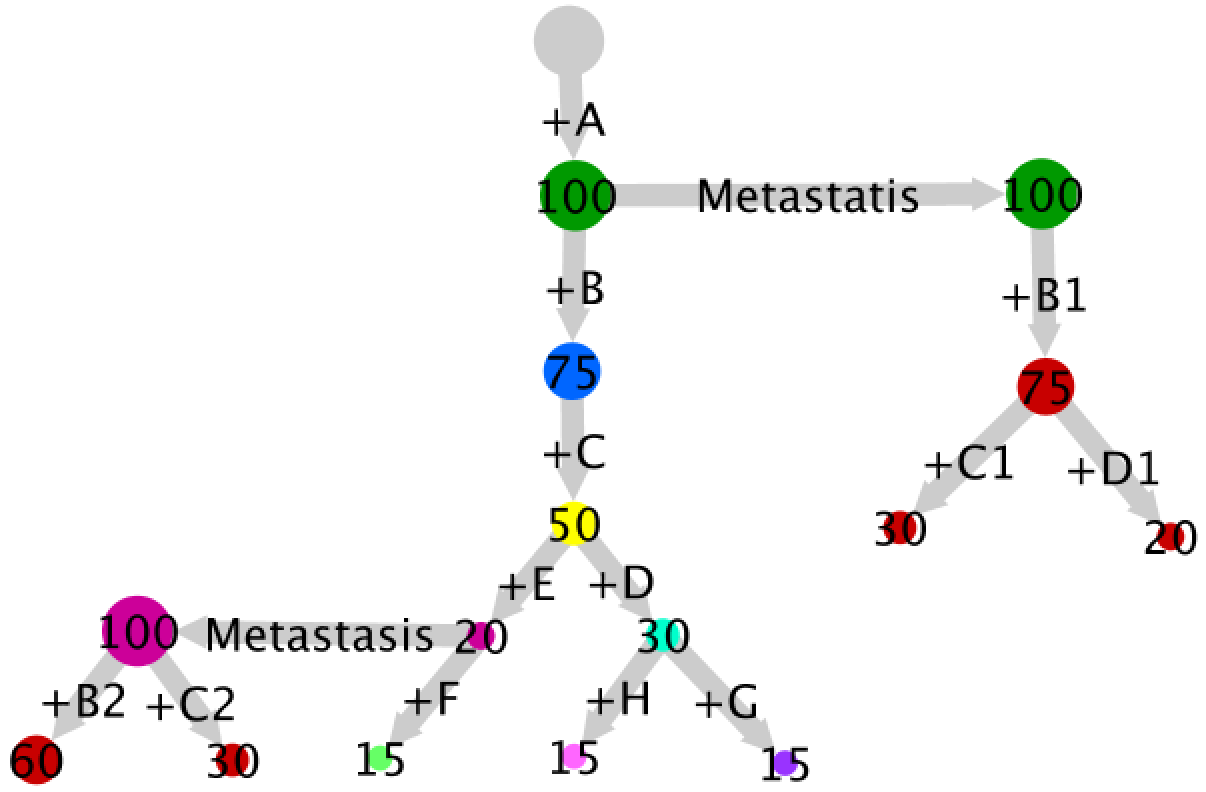
\includegraphics[width = 1.0\linewidth, trim={0 0 0 0}, clip=true]{metastasis_tree.png}
		%\subcaption{}
		%\label{}	
	\end{subfigure}%
\caption{Clonal evolution tree extended by an early (right) and late (left) metastatic tree. Nodes in the original tree are coloured as in figure \ref{fig:ce1tree}. All metastatic nodes are coloured red apart from the seeding clone which is coloured as in the base tree. Numbers on nodes indicate the CCF in that tumor of the most recently acquired mutation. Node size is a monotonically increasing function of this value.}
\label{fig:metatree}
\end{figure}

In the early metastatic tumor (tumor 1), the only mutation present from the original tumor (tumor 0) is mutation A. All other mutations arised later in the phylogenetic tree of tumor 0, and since we assume that the same mutation does not arise twice these mutations will not be present in tumor 1; i.e. they have a CCF of 0\% in tumor 1. Conversely, the mutations that arose in tumor 1 after metastasis will not be present in tumor 0 and thus have a CCF of 0\% in tumor 0.

This is illsutrated in figure \ref{fig:early} where we see that the 7 later mutations in tumor 0 (coloured; three of these are overlapping) all have CCFs of 0\% in tumor 1 while mutations B1, C1 and D1 arising in the metastatic tumor all have CCFs of 0\% in the original tumor. When plotting the CCFs of the original vs metastatic tumor, an early metastasis is thus characterized by many mutations occurring on the primary axes with a CCF of 0\% in one of the two tumors.


\begin{figure}[h]
	\centering
	\begin{subfigure}[t]{0.30\linewidth}
		\centering
		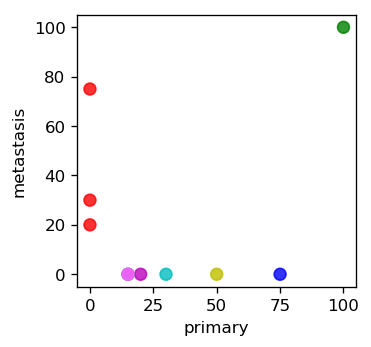
\includegraphics[width = 1.0\linewidth, trim={0 0 0 0}, clip=true]{meta_early.png}
		\subcaption{Early metastasis}
		\label{fig:early}	
	\end{subfigure}%
	\hspace{0.12 \linewidth}
	\begin{subfigure}[t]{0.30\linewidth}
		\centering
		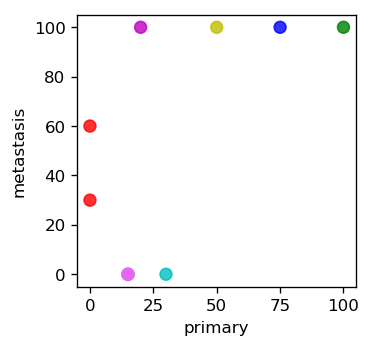
\includegraphics[width = 1.0\linewidth, trim={0 0 0 0}, clip=true]{meta_late.png}
		\subcaption{Late metastasis}	
		\label{fig:late}
	\end{subfigure}%
\caption{Plots showing the CCF in both the original tumor and an early (left) or late (right) metastatic tumor of mutations occurring in the original (coloured) or metastatic (red) tumor.}
\label{fig:metastases}
\end{figure}

Conversely in the late metastatic tumor (tumor 2), all mutations present in the seeding cell $ABCE$ will have a CCF of 100\% in the metastatic tumor (figure \ref{fig:late}). The late metastatic tumor is thus characterized by having multiple mutations which have CCFs of 100\% in the metastatic tumor despite having less than 100\% CCF in the original tumor. In the early metastasis in figure \ref{fig:early}, the only mutation with 100\% CCF is the seeding mutation $A$. In the late metastatic tumor, the mutations arising after metastasis in either tumor 0 or tumor 2 will still have a CCF of 0\% in the opposite tumor. In the case of polyclonal seeding, we can observe more complex CCF patterns with mid-range CCF values in both the primary and metastatic tumor, but that is not considered further in this report.

\newpage

\section*{Appendix}

This appendix includes all code used for the assignment\\
~\\

\lstinputlisting[language=python]{plot_data.py}

~\\

\lstinputlisting[language=python]{plot_pyclone.py}

~\\

\lstinputlisting[language=R]{run_ccube.r}

~\\

\lstinputlisting[language=python]{generate_data.py}

~\\

\lstinputlisting[language=python]{metastasis.py}



\end{document}

